% TOLL: Tolled One-way Lanes for Lifelong MAPD
%
% Build with:   python3 tools/build_docs.py paper
% or directly:  latexmk -lualatex -interaction=nonstopmode docs/latex/toll.tex
%
% LuaLaTeX rather than pdfLaTeX, because the worked-example boxes are verbatim
% transcripts of program output and contain box-drawing characters and Greek
% letters that only a Unicode engine with a real font can typeset.
%
% The five "Worked example" boxes are GENERATED. Everything between a
% "% worked-example: name" marker and its "% /worked-example" is written by
% tools/worked_examples.py from a live, seeded run, and tests/test_worked_examples.py
% fails if this file and the code disagree. Do not hand-edit inside a marker;
% run  python3 tools/worked_examples.py --write  instead.

\documentclass[11pt,a4paper]{article}

% Preamble for spar.tex. LuaLaTeX only.

\usepackage{geometry}
\geometry{a4paper, margin=27mm, top=25mm, bottom=27mm}

\usepackage{fontspec}
\usepackage{unicode-math}
% amssymb is deliberately absent: unicode-math provides the same symbols and
% the two clash over \eth and friends.
\usepackage{amsmath}
\usepackage{amsthm}
\setmonofont{DejaVu Sans Mono}[Scale=MatchLowercase]

% Stray Unicode in prose: the source of this document was Markdown that wrote
% Greek letters and arrows literally, and a missing glyph in the main roman
% font is silent. Mapping them here means a literal alpha typesets as maths
% rather than vanishing.
\usepackage{newunicodechar}
\newunicodechar{α}{\ensuremath{\alpha}}
\newunicodechar{β}{\ensuremath{\beta}}
\newunicodechar{γ}{\ensuremath{\gamma}}
\newunicodechar{δ}{\ensuremath{\delta}}
\newunicodechar{ε}{\ensuremath{\varepsilon}}
\newunicodechar{ζ}{\ensuremath{\zeta}}
\newunicodechar{η}{\ensuremath{\eta}}
\newunicodechar{λ}{\ensuremath{\lambda}}
\newunicodechar{μ}{\ensuremath{\mu}}
\newunicodechar{ν}{\ensuremath{\nu}}
\newunicodechar{ξ}{\ensuremath{\xi}}
\newunicodechar{ρ}{\ensuremath{\rho}}
\newunicodechar{σ}{\ensuremath{\sigma}}
\newunicodechar{τ}{\ensuremath{\tau}}
\newunicodechar{ω}{\ensuremath{\omega}}
\newunicodechar{Δ}{\ensuremath{\Delta}}
\newunicodechar{Σ}{\ensuremath{\Sigma}}
\newunicodechar{≤}{\ensuremath{\leq}}
\newunicodechar{≥}{\ensuremath{\geq}}
\newunicodechar{≠}{\ensuremath{\neq}}
\newunicodechar{≈}{\ensuremath{\approx}}
\newunicodechar{→}{\ensuremath{\rightarrow}}
\newunicodechar{←}{\ensuremath{\leftarrow}}
\newunicodechar{×}{\ensuremath{\times}}
\newunicodechar{·}{\ensuremath{\cdot}}
\newunicodechar{−}{\ensuremath{-}}
\newunicodechar{∈}{\ensuremath{\in}}
\newunicodechar{∅}{\ensuremath{\emptyset}}
\newunicodechar{∞}{\ensuremath{\infty}}

\usepackage{microtype}
% This document is full of long unbreakable identifiers (maximum_aisle_lock_time,
% congestion_assignment_only). Without room to stretch, a paragraph carrying two
% of them overflows the column.
\emergencystretch=3em
\tolerance=1200
\usepackage{booktabs}
\usepackage{longtable}
\usepackage{array}
\usepackage{multirow}
\usepackage{graphicx}
\graphicspath{{../figures/}}
\usepackage{float}
\usepackage[font=small,labelfont=bf]{caption}
\usepackage{enumitem}
\setlist{itemsep=0.25em, topsep=0.35em, parsep=0pt}

\usepackage{xcolor}
\definecolor{rulegrey}{HTML}{D6DBE4}
\definecolor{inkblue}{HTML}{1F4E79}
\definecolor{boxbg}{HTML}{F4F6FA}
\definecolor{ledebg}{HTML}{EFF5EF}
\definecolor{warnbg}{HTML}{FBF3EC}

\usepackage[most]{tcolorbox}
\tcbuselibrary{breakable}

\usepackage{algorithm}
\usepackage{algpseudocode}
\algrenewcommand\algorithmicrequire{\textbf{Input:}}
\algrenewcommand\algorithmicensure{\textbf{Output:}}
\floatname{algorithm}{Algorithm}

% Verdict marks. The results tables are read by people who want the answer
% before the argument, so every comparison carries a word and a glyph, never a
% colour alone.
\usepackage{pifont}
\definecolor{winc}{HTML}{18762F}
\definecolor{lossc}{HTML}{B3261E}
\definecolor{opencolour}{HTML}{9A6700}
\newcommand{\wins}{\textcolor{winc}{\ding{51}}}
\newcommand{\loses}{\textcolor{lossc}{\ding{55}}}
\newcommand{\unclear}{\textcolor{opencolour}{\ding{110}}}
% throughput, always reported per 1000 timesteps: 149 rather than 0.149
\newcommand{\tput}[1]{#1}

\usepackage[round,authoryear]{natbib}
\usepackage[hidelinks,bookmarks=true,bookmarksnumbered=true]{hyperref}
\hypersetup{
  pdftitle={SPAR: Soft-Priced Aisle Reversal},
  pdfsubject={Multi-agent pickup and delivery},
  colorlinks=true, linkcolor=inkblue, citecolor=inkblue, urlcolor=inkblue,
}
\usepackage{cleveref}

% ---------------------------------------------------------------------------
% editorial devices carried over from the Markdown guide
% ---------------------------------------------------------------------------

% "In one sentence" -- the one-line summary every system section opens with,
% so the document can be skimmed at one level and read at another.
\newtcolorbox{lede}{
  breakable, enhanced, colback=ledebg, colframe=ledebg!60!black,
  boxrule=0pt, leftrule=2pt, arc=0pt, outer arc=0pt,
  left=8pt, right=8pt, top=6pt, bottom=6pt,
  fontupper=\small\itshape,
}

% A generated worked example. Everything inside one of these is written by
% tools/worked_examples.py; see the header of spar.tex.
\newtcolorbox{workedexample}{
  breakable, enhanced, colback=boxbg, colframe=rulegrey,
  boxrule=0.6pt, arc=1.5pt,
  left=8pt, right=8pt, top=7pt, bottom=7pt,
  fontupper=\small,
}

% A finding that contradicts the design, or a caveat a reader must carry.
\newtcolorbox{caveat}[1][]{
  breakable, enhanced, colback=warnbg, colframe=warnbg!55!black,
  boxrule=0pt, leftrule=2pt, arc=0pt, outer arc=0pt,
  left=8pt, right=8pt, top=6pt, bottom=6pt,
  fontupper=\small, #1
}

% The answer before the argument: one box per section that has a headline
% finding, stating it in the fewest words that remain true.
\definecolor{verdictbg}{HTML}{EEF3FA}
\newtcolorbox{verdict}[1][The short answer]{
  breakable, enhanced, colback=verdictbg, colframe=inkblue,
  boxrule=0pt, leftrule=3pt, arc=0pt, outer arc=0pt,
  left=9pt, right=9pt, top=7pt, bottom=7pt,
  fonttitle=\small\bfseries, title={#1}, coltitle=inkblue,
  attach title to upper={\par\vspace{3pt}},
}

% Fixed-width transcripts (ASCII diagrams, generated tables) that must not
% reflow. \small is deliberate: these are program output, not prose.
\newenvironment{transcript}
  {\begin{quote}\small\ttfamily\obeylines\obeyspaces\parskip=0pt}
  {\end{quote}}

\newcommand{\code}[1]{\texttt{#1}}
\newcommand{\param}[1]{\texttt{#1}}
\newcommand{\variant}[1]{\texttt{#1}}
% the indicator function. \mathbf rather than \mathbbm: unicode-math has no
% blackboard digit, and a bold 1 is unambiguous next to the weights.
\newcommand{\ind}[1]{\mathbf{1}\!\left[#1\right]}

% notation shorthands used throughout
\newcommand{\Dg}[1]{D_{#1}}
\newcommand{\pos}[2]{x_{#1}(#2)}
\newcommand{\score}{S_i(v)}
\newcommand{\INF}{\ensuremath{\infty}}

\setcounter{tocdepth}{2}
\setcounter{secnumdepth}{3}

\theoremstyle{definition}
\newtheorem{proposition}{Proposition}


\title{\textbf{TOLL}\\[0.2em]
  \large \textnormal{\textbf{T}olled \textbf{O}ne-way \textbf{L}anes for
  \textbf{L}ifelong pickup-and-delivery}\\[0.55em]
  \large Direction as a price, not a rule}
\author{}
\date{}

\begin{document}

\maketitle
\thispagestyle{empty}

\begin{abstract}
\noindent
Lifelong multi-agent pickup and delivery (MAPD) in a warehouse is dominated by
a single structural fact: the map has narrow aisles, and traffic in a narrow
aisle interferes with itself. \emph{Priority Inheritance with Backtracking}
(PIBT) handles that interference locally and cheaply --- a blocked robot lends
its priority to the robot in its way and asks it to move --- but it plans one
timestep at a time and has no notion of an aisle at all. The obvious extension
is to give aisles directions, as a warehouse floor manager would: make a
contended corridor one-way while the traffic in it is one-way.

This document describes \textbf{TOLL} --- \emph{Tolled One-way Lanes for
Lifelong pickup-and-delivery} --- and its planner \textbf{TOLL-PIBT}, and
reports what happened when it was measured. The name is the claim: a robot may
drive the wrong way down a one-way aisle, and pays a toll for doing so. Its central design decision is negative and, we
argue, general: a one-way rule must enter the planner as a \textbf{term in the
objective}, never as a \textbf{constraint on the domain}. Deleting a
counterflow move from a robot's candidate set --- the natural implementation,
and the one the original specification called for --- destroys the property
priority inheritance runs on, namely that a robot can always be pushed
somewhere. Pricing the same move instead, at a cost above every other soft
preference and below the value of a step of progress, preserves it. Measured
this single distinction is worth between $1.9\times$ and $3.7\times$
throughput on every map where an aisle ever commits a direction, and is the
largest effect in the system. Two further
mechanisms follow from the same reasoning: an aisle signal needs a maximum
green as well as a minimum, or a balanced warehouse starves half its traffic;
and deadlock recovery must require a corroborated stall signal, or it spends
its time dismantling ordinary queues.

We evaluate against two published lifelong baselines --- Token Passing and
RHCR --- and against every ablation of the method itself, with bootstrap
confidence intervals and permutation tests over five seeds. The result is
scoped rather than universal, and we report it that way. Against both external
baselines TOLL wins decisively and significantly on every map tested, at a
twentieth to a three-hundredth of their cost per timestep. Against plain
lifelong PIBT its aisle layer is ahead by 21--27\% on the two aisle-shaped maps
and behind by 18--19\% on the two open ones --- and at five seeds the losses
are significant while the wins ($p = 0.056$ and $0.063$) are not yet. The
mechanisms above are, wherever their mechanism can act at all. The final
sections say exactly where that boundary falls, and what it would take to
settle the part that is still open.
\end{abstract}

\vfill

\begin{center}
\small
Source, simulator and every number in this document:
\url{https://github.com/sinayanaik/aisleflow}\\
Figures regenerate from \texttt{docs/data/}; worked examples regenerate from the code.\\[0.4em]
\footnotesize
The repository and the Python package predate this name and still read
\texttt{aisleflow} and \texttt{lda\_pibt}; \texttt{TOLL} and
\texttt{TOLL-PIBT} are the method and its planner throughout this document.
\end{center}

\clearpage
\tableofcontents
\clearpage

\part{The method}

\section{The problem, stated precisely}
\label{sec:problem}

\begin{lede}
A warehouse floor, a never-ending stream of jobs, and a fleet that must keep
moving forever. This section fixes the model, the constraints and --- the part
that decides how every later number should be read --- the traffic regime the
measurements are taken in.
\end{lede}

\subsection{Environment and agents}

The warehouse is a 4-connected grid graph $G = (V, E)$. A vertex is a cell
$v = (r, c)$; $V$ holds the passable cells and $E$ joins orthogonally adjacent
ones. Shelving, walls and racking are simply absent from $V$. Certain vertices
carry a role: $V_{\mathrm{p}} \subset V$ are pickup stations,
$V_{\mathrm{d}} \subset V$ delivery stations, and $V_{\mathrm{k}} \subset V$
parking bays.

A fleet $A = \{1, \dots, n\}$ of identical robots occupies distinct vertices.
Time is discrete and synchronous: at each timestep every robot simultaneously
either moves to a vertex adjacent to its current one or stays where it is,
\begin{equation}
  \pos{i}{t+1} \in N(\pos{i}{t}) \cup \{\pos{i}{t}\},
  \label{eq:move}
\end{equation}
and a joint move is legal exactly when it creates neither of the two standard
conflicts:
\begin{align}
  \text{vertex conflict:} && \pos{i}{t+1} &= \pos{j}{t+1}, & i &\neq j,
  \label{eq:vertex-conflict}\\
  \text{swap conflict:} && \pos{i}{t+1} = \pos{j}{t} &\ \wedge\
    \pos{j}{t+1} = \pos{i}{t}, & i &\neq j.
  \label{eq:swap-conflict}
\end{align}
There is no rotation cost and no kinematic model; a robot's heading is tracked
only so that changing it can be discouraged (\Cref{sec:score-turn}).

\subsection{The task stream}

This is a \emph{lifelong} problem, not a one-shot one. Tasks are not known in
advance and never stop arriving. A task $\tau = (p, d, t_{\mathrm{rel}})$
releases at time $t_{\mathrm{rel}}$ and requires some robot to visit its pickup
$p \in V_{\mathrm{p}}$ and then its delivery $d \in V_{\mathrm{d}}$, in that
order. Arrivals follow one of four processes (\Cref{sec:arrivals}); the
experiments in this document use a Poisson process of mean rate $\lambda$
tasks per timestep.

A robot is assigned at most one task at a time and is free again on delivery.
Assignment is itself part of the problem --- which robot takes which job
matters --- and is handled by a greedy minimum-cost match
(\Cref{sec:assignment}) held \emph{identical} across every planner compared in
this document, so that comparisons isolate the movement layer.

The quantity a task contributes to the evaluation is its \emph{service time},
\begin{equation}
  \mathrm{svc}(\tau) = t_{\mathrm{complete}}(\tau) - t_{\mathrm{rel}}(\tau),
\end{equation}
defined only for tasks that actually complete --- a restriction
\Cref{sec:regime} returns to, because it is the single most misread number in
the whole evaluation.

\subsection{Objective}

Over a horizon of $T$ timesteps, with $K$ tasks completed, the primary
objective is \textbf{throughput}
\begin{equation}
  \Theta = \frac{K}{T} \quad \text{(tasks per timestep)},
  \label{eq:throughput}
\end{equation}
subject to the joint plan being conflict-free at every step. Makespan --- the
standard objective for one-shot MAPF --- is undefined here: there is no last
task. Sum-of-costs is likewise unavailable, since the set of costs is not
fixed in advance.

Secondary quantities are reported throughout, and each answers a different
question: mean and $p_{95}$ service time (latency, and tail latency),
Jain's fairness index over per-robot completion counts (is the fleet used
evenly), direction switches per 1000 steps (is the aisle signal stable),
head-on conflicts and counterflow moves (is the aisle layer doing what it
claims), and mean planner runtime per timestep (what the method costs).

\subsection{The traffic regime, and why it decides how to read every number}
\label{sec:regime}

The measurements in this document are taken in \textbf{saturation}, and this
must be stated before any of them is quoted.

The arrival rate $\lambda$ is set well above what the floor can serve. On
\variant{warehouse\_medium} tasks arrive at $\lambda = 1.5$ per timestep and
the best configuration completes about $0.50$ per timestep; on
\variant{warehouse\_bottleneck}, $\lambda = 0.8$ against $0.15$ served. Between
an eighth and a third of offered demand is served (\Cref{tab:scenarios}); the
backlog grows without bound for the whole run. Three consequences follow, and all three are
routinely misread.

\begin{enumerate}
\item \textbf{Throughput measures capacity, not effort.} In saturation there
is always another task waiting, so no planner is ever idle for want of work and
$\Theta$ is exactly the floor's service capacity under that planner. This is
why $\Theta$ is the primary objective and why differences in it are meaningful
even when they look small: $0.50$ against $0.31$ tasks per timestep is a $61\%$
difference in the capacity of the warehouse.

\item \textbf{Service time is censored, and the censoring is not random.}
$\mathrm{svc}(\tau)$ exists only for completed tasks. A planner that serves
only the nearby, easy tasks and abandons the rest reports an \emph{excellent}
mean service time. This is not hypothetical: on
\variant{warehouse\_bottleneck} Token Passing reports a mean service time of
$31$ timesteps --- against $154$ for the planner that delivers twenty times as
many tasks --- because the handful of tasks it finishes are the ones it
finishes in the first few timesteps, before the corridor jams for good. Mean
service time may be compared only between planners with comparable throughput.
\Cref{fig:censoring} shows this trap directly.

\item \textbf{Robot count is not a free parameter.} All planners are compared
at the same fleet size on the same map, because throughput is not monotone in
fleet size once the floor is congested --- adding robots past the congestion
knee lowers it.
\end{enumerate}

\begin{caveat}
Every table in \Cref{sec:results} therefore reports throughput first, quotes
service time only alongside it, and never ranks two planners by service time
alone. A reader who takes one thing from this section: \emph{a low mean service
time next to a low throughput is a symptom, not an achievement.}
\end{caveat}

\subsection{What makes this hard, in one paragraph}

A warehouse map is mostly corridors. In a single-file corridor, two robots
wanting opposite directions cannot both proceed, and no local rule that treats
them symmetrically resolves it; one must yield, and something must decide
which. Worse, in a lifelong setting the pair that meets head-on is replaced by
another pair a few timesteps later, so a resolution that works once must keep
working forever, under an adversarial arrival process the planner does not
control. Optimal joint planning would resolve this and is exponential
(\Cref{sec:related-cbs}); planning each robot independently against a
reservation table is cheap and deadlocks (\Cref{sec:related-tp}). The
interesting region is between the two, and that is where PIBT
(\Cref{sec:related-pibt}) and this work sit.

\section{Prior methods, and how each one fails here}
\label{sec:related}

\begin{lede}
Four families of solution, in increasing order of how much they give up for
speed. Each is described by what it optimises, what one timestep costs it, and
the specific way it breaks in a narrow lifelong warehouse --- because that
failure mode is what the next section is designed around.
\end{lede}

\subsection{Optimal MAPF: CBS and its relatives}
\label{sec:related-cbs}

Conflict-Based Search \citep{sharon2015cbs} solves one-shot MAPF optimally with
a two-level search: a low level plans each agent independently, and a high
level branches on the first conflict found between two agents' paths, adding a
constraint forbidding one of them from the conflicting vertex or edge at that
time and replanning only that agent. It is complete and optimal for sum-of-costs,
and it is exponential in the number of conflicts --- which in a dense warehouse
corridor is very nearly the number of agent pairs.

Two properties disqualify it as-is here. First, cost: the high-level tree grows
with contention, and contention is exactly the condition of interest. Second,
and more fundamental, CBS answers a one-shot question. In a lifelong setting
goals change continuously, so the plan CBS produces is stale before it is
finished. Every practical lifelong system built on CBS therefore truncates it,
which is what RHCR does.

\subsection{PIBT: one timestep, decided locally}
\label{sec:related-pibt}

Priority Inheritance with Backtracking \citep{okumura2019pibt} abandons
multi-step planning entirely. At every timestep, robots are considered in
descending priority order; each takes the best-scoring legal move available to
it. If the cell it wants is occupied by a robot that has not yet decided, the
requesting robot \emph{lends its priority} to the occupant and asks it to move
first --- recursively. If the occupant can find no legal move, the request
backtracks and the requester tries its next candidate. \Cref{sec:pibt} gives
the recursion in full.

Two properties matter for everything that follows.

\begin{enumerate}
\item \textbf{Cost.} One timestep is $O(|A|(\Delta(G) + F + \log|A|))$ for a
fleet $A$, maximum degree $\Delta(G)$ and per-candidate scoring cost $F$. On
the maps used here this is 0.4--1.0\,ms per step, one to two orders of
magnitude below either baseline in \Cref{sec:results}.

\item \textbf{The push property.} Priority inheritance works because a robot
asked to move can, in general, be pushed somewhere. PIBT's progress guarantee
is proved under the assumption that every edge of $G$ lies on a simple cycle;
informally, a robot displaced from a cell always has an alternative. This
assumption is not a technicality --- \Cref{sec:contribution-soft} shows that
the natural way to implement one-way aisles \emph{violates it by construction},
and that this, rather than anything about direction control as an idea, was the
cause of every collapse previously attributed to the aisle layer.
\end{enumerate}

What PIBT does not have is any notion of structure above a single cell. It
cannot know that a corridor is a corridor, cannot commit a corridor to one
direction, and cannot coordinate two robots that will meet in ten timesteps.
Every robot's decision is local and one step deep. That is the gap this work
addresses.

\subsection{Token Passing: reserve a path, or wait}
\label{sec:related-tp}

Token Passing \citep{ma2017tp} is the standard lifelong-MAPD baseline for
exactly this pickup-and-delivery setting. A token circulates; a robot holding
it plans a collision-free path to its goal through a shared reservation table
using cooperative A$^\ast$ over $(\text{vertex}, \text{time})$ states, commits
that path into the table, and passes the token on. A robot that cannot find a
path waits in place.

Its failure mode in a narrow warehouse is structural, not a matter of tuning:
\textbf{Token Passing has no mechanism by which a blocked robot can displace
the robot blocking it}. Once robots queue nose-to-tail in a single-file
corridor, no robot in the queue can reserve a path through the robots ahead of
it, every robot's search fails, every robot waits, and the configuration is
absorbing --- it never resolves for the rest of the run. On
\variant{warehouse\_bottleneck}, whose two halves are joined by one corridor,
all 16 robots reach this state and the run completes essentially no tasks. The
first comparison animation in \code{docs/gifs/} shows precisely this, beside
the same scenario under priority inheritance.

This is the failure PIBT was invented to remove, and it is worth being explicit
that observing it here is a confirmation of the published analysis rather than
a criticism of Token Passing: the algorithm was never claimed to be live in
maps without alternative routes.

\subsection{RHCR: rolling-horizon windowed CBS}
\label{sec:related-rhcr}

Rolling-Horizon Collision Resolution \citep{li2021rhcr} makes CBS lifelong by
bounding it in time. Every \param{replan\_period} timesteps all robots are
jointly replanned over a window of \param{window} timesteps using CBS
restricted to that window; conflicts beyond the window's edge are simply not
resolved yet, on the reasoning that they will be replanned before they arrive.
Between replans, individual stale paths are repaired.

RHCR is the strongest of the three published methods for this setting and its
design target is large: hundreds of robots on warehouses far bigger than the
ones used here, where a rolling horizon pays for itself against full CBS. At
the scale measured in this document, with untuned window parameters
($10/5$), it costs 43--98\,ms per timestep --- against 0.4--4.4\,ms for the
PIBT variants --- and does not convert that cost into throughput. We report
this as a property of \emph{this baseline at this scale with these defaults}
and not as a claim about RHCR generally; \Cref{sec:results-caveats} states the
caveat again where the numbers appear.

\subsection{Directional and structural traffic control}
\label{sec:related-directional}

Making corridors one-way is not a new idea; warehouse floors have been run that
way by human traffic rules for as long as there have been warehouses, and
highway-style directional layouts appear throughout the MAPF and AGV
literature. The design decisions that distinguish proposals are: at what
granularity a direction is decided (a whole map, a corridor, an edge), how
often it may change, and --- the question this work turns out to hinge on ---
\textbf{what a committed direction does to a move that opposes it}.

The usual answer is that it forbids it. A one-way corridor is one-way; a move
against it is not legal; the planner never sees it. Under a planner that plans
whole paths, this is harmless: the path simply routes around. Under PIBT it is
not harmless at all, for the reason given in \Cref{sec:related-pibt}, and that
is the subject of the next section.

\section{What TOLL-PIBT changes, and why it is different}
\label{sec:contribution}

\begin{lede}
Four changes, three of them consequences of one idea: a high-level traffic
rule may reorder what a local planner considers, and must never remove it.
Each is stated as an inequality or a property, with the measurement that tests
it.
\end{lede}

The architecture is two layers, and the division between them is the whole
design (\Cref{sec:architecture}). The upper layer decides what each robot
\emph{wants}: which task, which waypoint, which route, which direction its
aisle should be flowing, who plans first. The lower layer --- PIBT, unmodified
--- decides what is \emph{allowed}. The upper layer may rank the lower layer's
options. It may not delete them. Everything below follows from taking that
sentence literally.

\subsection{Direction as a term in the objective, not a constraint on the domain}
\label{sec:contribution-soft}

\subsubsection{The two implementations}

Let $C_i = N(\pos{i}{t}) \cup \{\pos{i}{t}\}$ be robot $i$'s candidate set and
let $\mathrm{safe}_i(v)$ hold when moving to $v$ creates neither conflict of
\Cref{eq:vertex-conflict,eq:swap-conflict}. Write
$\mathrm{opp}_i(v)$ for the predicate ``moving to $v$ opposes the committed
direction of the aisle being entered'' (\Cref{sec:aisle-legality}). The two
ways to enforce a one-way rule are:
\begin{align}
  F^{\mathrm{hard}}_i &= \{\, v \in C_i \;:\; \mathrm{safe}_i(v) \wedge \neg\,\mathrm{opp}_i(v) \,\},
  \label{eq:hard}\\
  F^{\mathrm{soft}}_i &= \{\, v \in C_i \;:\; \mathrm{safe}_i(v) \,\},
  \qquad
  \score \;\mathrel{-}=\; \zeta \cdot \ind{\mathrm{opp}_i(v)}.
  \label{eq:soft}
\end{align}
\Cref{eq:hard} is what the original specification for this system called for,
and what a one-way rule ordinarily means. \Cref{eq:soft} is what TOLL-PIBT
does: the move stays in the set, sorted to the back, and is taken when nothing
better is available.

\subsubsection{Why the difference is not cosmetic}

Under a path planner the two are nearly equivalent --- a forbidden edge simply
raises the cost of the route through it, and the planner routes around. Under
PIBT they are not, because PIBT's mechanism for resolving a blockage is to
\emph{push}, and pushing needs somewhere to push to.

\begin{proposition}[Candidate preservation]
\label{prop:preservation}
For every robot $i$ and timestep $t$, $F^{\mathrm{hard}}_i \subseteq
F^{\mathrm{soft}}_i$, and $F^{\mathrm{soft}}_i$ is exactly the set PIBT would
have without any aisle layer at all. Consequently every joint move reachable
under \Cref{eq:hard} is reachable under \Cref{eq:soft}, and the aisle layer
under \Cref{eq:soft} cannot reduce the set of configurations the planner can
escape from.
\end{proposition}

The converse fails, and it fails exactly where it hurts. Consider a
single-file aisle $a = (u_1, \dots, u_m)$ committed \textsc{forward}
(increasing index), occupied by robots $i_1, \dots, i_m$, one per cell, with
$u_m$'s forward neighbour occupied by a robot that cannot move this timestep.
Under \Cref{eq:hard}, each $i_k$ has exactly two candidates: $u_{k+1}$, which
is occupied, and staying put; the reverse move $u_{k-1}$ has been deleted.
Priority inheritance therefore walks the chain $i_1 \to i_2 \to \dots \to i_m$,
finds no robot with a free legal move, backtracks all the way, and every robot
stays. The configuration is unchanged next timestep, and the timestep after
that. Under \Cref{eq:soft}, $i_1$ retains $u_0$ at a cost of $\zeta$, the chain
terminates by pushing one robot backwards out of the aisle, and the aisle
drains.

This is not a hypothetical. Instrumented on \variant{warehouse\_corridors}
under \Cref{eq:hard}: all 35 robots stalled by $t = 120$, four aisles locked
\textsc{reverse}, the identical global state still present at $t = 199$. The
second comparison animation in \code{docs/gifs/} is this pair of runs side by
side.

\subsubsection{Sizing \texorpdfstring{$\zeta$}{zeta}}
\label{sec:contribution-zeta}

Pricing only works if the price is right. The candidate score
(\Cref{sec:score-full}) is
\begin{multline}
  \score = \underbrace{\alpha \cdot \mathrm{progress}}_{\alpha = 10}
    + \underbrace{\beta_i \cdot \ind{\text{preferred direction}}}_{\beta \leq 3}
    + \underbrace{\gamma_i \cdot \ind{\text{stays in aisle}}}_{\gamma \leq 2}
    - \underbrace{\lambda_{\mathrm{turn}} P_{\mathrm{turn}}}_{\leq 1}\\
    - \underbrace{\mu C_i(v)}_{\leq 1}
    - \underbrace{\nu P_{\mathrm{wait}}}_{\leq 0.2}
    - \underbrace{\xi \ind{\text{bottleneck}}}_{\leq 1}
    - \underbrace{\zeta \ind{\mathrm{opp}_i(v)}}_{\zeta = 8},
\end{multline}
and $\zeta$ is placed by two inequalities.

\paragraph{$\zeta < \alpha$: progress can still buy its way through.}
A counterflow move that closes one step of distance scores
$\alpha - \zeta = +2$ before minor terms; staying in place scores
$-\nu = -0.2$. So a robot in a corridor whose only progressing move is against
the flow \emph{takes it}, and pays. This is the inequality that makes
\Cref{prop:preservation} operational rather than merely set-theoretic: the
retained candidate is not just present, it is reachable.

\paragraph{$\zeta$ above every other preference: direction still governs.}
Individually, $\zeta = 8$ exceeds the largest competing soft term
($\beta_{\max} = 3$) by $2.7\times$, and exceeds the sum of both positive
preference terms ($\beta + \gamma = 5$). It does not exceed the arithmetic sum
of all six non-progress terms at their simultaneous extremes ($8.2$), and we
state that plainly rather than claiming a domination that the numbers do not
support: the guarantee is that no ordinary combination of preferences reverses
a direction decision, not that no contrived one can. What is guaranteed
exactly is the ordering against progress, above.

\subsubsection{What it is worth}

Single-factor comparisons (\code{config.PAIRED\_DESIGNS}), same seeds, same
maps, the same direction decisions, differing only in \Cref{eq:hard} versus
\Cref{eq:soft}: $1.9\times$ throughput on \variant{warehouse\_corridors},
$2.5\times$ on \variant{warehouse\_medium} and $3.7\times$ on
\variant{warehouse\_narrow}, each at $p = 0.008$ --- the floor of a five-seed
permutation test --- and up to $4.6\times$ with entry admission also enabled.
On \variant{warehouse\_bottleneck} the two arms are identical, because no aisle
there ever commits a direction and the treatment has nothing to change.

It is the largest single effect measured anywhere in this system. \Cref{fig:forest} plots it beside every other
mechanism, and \Cref{sec:results-mechanisms} gives the table.

\begin{caveat}
The general form of this finding is worth stating separately from TOLL-PIBT,
because it applies to any local, push-based planner: \emph{a traffic rule
imposed as a hard constraint removes the freedom that local conflict resolution
runs on.} If the planner resolves blockages by displacement, every constraint
that shrinks the candidate set shrinks the set of blockages it can resolve.
Price the rule instead, above the preferences and below the objective.
\end{caveat}

\subsection{The aisle as a traffic signal: a maximum green, not only a minimum}
\label{sec:contribution-maxgreen}

An aisle decides its direction from the aggregate demand of the robots routed
through it, $S_a^{+}$ forward and $S_a^{-}$ reverse
(\Cref{sec:aisle-demand}), and commits when the imbalance leaves a dead band:
\begin{equation}
  \text{commit \textsc{forward} if } S_a^{+} - S_a^{-} > \tau_{\mathrm{switch}},
  \qquad
  \text{\textsc{reverse} if } S_a^{+} - S_a^{-} < -\tau_{\mathrm{switch}},
\end{equation}
with a minimum lock $T_{\min}$ after each commit. Hysteresis of this kind is
standard and it is only half a traffic signal: the dead band and the minimum
lock bound how \emph{soon} a direction may change, and nothing bounds how long
it may persist.

That gap is not a corner case in a warehouse; it is the normal operating
condition. Put pickups down one side of the floor and deliveries down the
other --- the standard layout, and three of the four maps used here --- and
loaded robots want one direction while empty robots want the other, in
near-equal measure. The imbalance sits inside the dead band forever, and an
aisle that committed a direction once holds it for the rest of the run while
half its traffic waits.

TOLL-PIBT adds a maximum green $T_{\max}$: past $T_{\max}$ steps in one
direction, \emph{any} opposing demand at all forces the aisle to drain and
flip. This gives a bounded-wait property that the dead band alone does not.

\begin{proposition}[Bounded direction wait]
\label{prop:maxgreen}
If an aisle $a$ holds direction $\delta$ from time $t_0$ and there is opposing
demand at every step, then $a$ commits $\bar{\delta}$ no later than
$t_0 + T_{\max} + T_{\mathrm{drain}}$, where $T_{\mathrm{drain}} \leq
\param{max\_drain\_time}$ is bounded because a \textsc{draining} aisle that has
not emptied within that many steps is force-reopened
(\Cref{sec:aisle-state-machine}).
\end{proposition}

Flips forced this way are counted separately as \code{starvation\_flips},
which keeps two questions apart that a single switch counter conflates: ``does
hysteresis stop oscillation?'' and ``does anybody starve?''

Measured, the maximum green is \emph{not} significant on throughput --- and
that is itself the finding. It was decisive while direction was a hard
constraint, because then a starved robot had no way out at all. Once
counterflow is merely expensive, a robot can buy its way out of a starved
aisle, so liveness no longer rests on the signal alone: the two fixes are
partly redundant. It stays enabled because it makes the aisle layer
\emph{correct} rather than merely survivable, and because its effect on
switching is significant: on \variant{warehouse\_narrow}, $22.5$ direction
switches per 1000 steps against $1.0$ without it ($p = 0.016$), of which $5.2$
per run are flips the rule forced rather than demand. Without it, those aisles
never turn at all. The third comparison animation shows
an aisle that never flips beside one that must.

\subsection{Recovery on corroborated stalls only}
\label{sec:contribution-corroboration}

A deadlock detector in a lifelong warehouse faces an unusual difficulty: in
saturation, the observable signature of a deadlock is also the observable
signature of a perfectly healthy queue. Three stall signals are available
(\Cref{sec:deadlock-signals}):
\begin{enumerate}
\item no route progress for $t_{\mathrm{blocked}}$ steps;
\item a cycle in the wait-for graph, where $i \to j$ when $i$'s
  priority-inheritance request went to $j$;
\item a repeated configuration --- the robot's last $k$ positions equal the $k$
  before them.
\end{enumerate}
Signal 1 alone describes every robot in every queue on a busy floor. Treating
it as sufficient means recovery fires constantly on healthy traffic, and
recovery's upper levels are drastic: temporary reverse movement, escape-vertex
assignment, waypoint hijack (\Cref{sec:recovery-levels}). Queues get taken
apart and rebuilt continuously.

TOLL-PIBT requires corroboration: a group must show signal 1 \emph{and} at least
one of signals 2 or 3 before escalation begins. Signals 2 and 3 are the ones
with a genuine deadlock semantics --- a circular wait, or a state the system
has demonstrably returned to. On \variant{warehouse\_corridors} this is worth
$0.134$ against $0.022$ tasks per timestep ($p = 0.008$), a six-fold difference
obtained entirely by declining to act on the weakest evidence. On the other
maps it points the same way without clearing five-seed significance. The fourth comparison
animation shows both.

There is a second-order lesson in how this defect stayed hidden. While
direction was a hard constraint, the architecture was manufacturing real
deadlocks continuously, so an over-eager detector looked useful: it \emph{was}
rescuing real deadlocks, of the system's own making. Fixing
\Cref{sec:contribution-soft} is what made the over-eagerness visible.

\subsection{Cost}
\label{sec:contribution-cost}

The aisle layer is a constant-factor addition to PIBT, not a change in its
complexity class. Per timestep, for fleet $A$ on graph $G$ with aisle set
$\mathcal{A}$:

\begin{table}[H]
\centering
\small
\begin{tabular}{@{}llr@{}}
\toprule
\textbf{Planner} & \textbf{Per-timestep cost} & \textbf{Measured (ms/step)} \\
\midrule
PIBT \citep{okumura2019pibt}
  & $O(|A|(\Delta(G) + F + \log|A|))$ & 0.4--1.0 \\
TOLL-PIBT (this work)
  & $+\,O(|A| + |\mathcal{A}|)$ aisle bookkeeping & 1.4--4.4 \\
Token Passing \citep{ma2017tp}
  & $O(|A| \cdot \mathrm{A}^\ast(|V| \cdot T_{\mathrm{horizon}}))$ & 32--222 \\
RHCR \citep{li2021rhcr}
  & windowed CBS, exponential in conflicts, capped & 43--98 \\
\bottomrule
\end{tabular}
\caption{Per-timestep cost. Measured columns are means over five seeds on the
three baseline maps of \Cref{sec:results}; the spread is across maps and fleet
sizes. The aisle layer costs a small constant factor over PIBT; both
path-planning baselines cost one to two orders of magnitude more.}
\label{tab:complexity}
\end{table}

The added work per timestep is: updating each aisle's demand sums
(one pass over robots), running the direction decision for each aisle (constant
work each), granting reservations in priority order (one pass), and the
deadlock detector's wait-for cycle search (linear in the fleet). None of it
involves a search, and none of it is repeated per candidate --- the congestion
and distance terms consumed by the score are precomputed or cached
(\Cref{sec:congestion,sec:graph-distances}), which is what keeps $F$ at $O(1)$.

\subsection{What this does not claim}
\label{sec:contribution-scope}

The honest summary, stated here rather than buried in \Cref{sec:results}: the
aisle layer is ahead where aisles are scarce and contended, and behind where
they are not. Against plain lifelong PIBT it gains 27\% on
\variant{warehouse\_bottleneck} and 21\% on \variant{warehouse\_corridors}, and
loses 18\% and 19\% on the two open maps --- and at five seeds \emph{the two
losses are significant and the two wins are not} ($p = 0.056$ and $0.063$
against $0.016$ and $0.008$). The fifth comparison animation is the losing
case, shown at the same size as the winning ones.

So the claim this document defends is precise: the mechanisms of this section
are established, the scoping of the aisle layer to aisle-shaped maps is
consistent and not yet significant, and \Cref{tab:honest} says which is which.


\part{The system, in full}

\section{The two-layer architecture}
\label{sec:architecture}

\begin{lede}
Every mechanism in this document sits in one of two layers: an upper layer that
decides what each robot \emph{wants}, and a lower layer that decides what is
\emph{allowed}. Only the lower layer can prevent a collision, and nothing in
the upper layer is permitted to remove a move the lower layer would have
considered.
\end{lede}

TOLL-PIBT extends PIBT \citep{okumura2019pibt} --- a single-timestep,
decentralised multi-agent collision-avoidance algorithm --- with a high-level
layer that decides \emph{what} each robot wants (task, waypoint, preferred
direction, priority) without ever touching collision safety.

\begin{center}
\small\ttfamily
\begin{tabular}{@{}l@{}}
\toprule
\textbf{\textsf{HIGH LEVEL}} \\
task stream $\rightarrow$ assignment $\rightarrow$ waypoints $\rightarrow$ routes $\rightarrow$ directional demand \\
$\rightarrow$ aisle direction (hysteresis, drain) $\rightarrow$ reservations \\
$\rightarrow$ priorities $\rightarrow$ deadlock detection \& local recovery \\
\midrule
\multicolumn{1}{@{}c@{}}{\textsf{\itshape ranks and prices candidates; never removes one}} \\
\midrule
\textbf{\textsf{LOW LEVEL (PIBT)}} \\
candidates $\rightarrow$ safety rejection $\rightarrow$ score-sorted $\rightarrow$ priority \\
inheritance $\rightarrow$ backtracking $\rightarrow$ one synchronised timestep \\
\bottomrule
\end{tabular}
\end{center}

The invariant this document keeps returning to: \textbf{everything above the
line only reorders candidate moves; only the PIBT recursion
(\Cref{sec:pibt}) and its validation companions (\Cref{sec:pibt-conflicts})
decide collision-freedom.} No high-level formula can, by construction, produce
two robots on the same vertex.

The middle row of that diagram is where this system differs from its own
original specification, and from the usual way a directional rule is
implemented. The specification listed ``violates aisle direction'' and
``violates a reservation'' among the low level's hard rejection rules; the same
document's design principle said the high level never replaces PIBT's
collision checks or its backtracking. Those two cannot both hold, and
\Cref{sec:contribution-soft} works out which one had to give.

\Cref{tab:modules} maps the sections that follow onto the code.

\begin{table}[H]
\centering\small
\begin{tabular}{@{}lll@{}}
\toprule
\textbf{Module} & \textbf{Section} & \textbf{What it does} \\
\midrule
\code{types.py} & --- & enums, \code{Vertex}, \code{Reservation} \\
\code{config.py} & \ref{sec:parameters} & \code{Params}, ablation presets, factorial designs \\
\code{graph.py} & \ref{sec:graph} & grid, BFS distance maps, articulation points, bridges \\
\code{warehouse.py} & \ref{sec:graph} & map parsing, vertex metadata, aisle segmentation \\
\code{task.py} & \ref{sec:robots-tasks} & tasks, queue, four arrival processes \\
\code{robot.py} & \ref{sec:robots-tasks} & robot state \\
\code{congestion.py} & \ref{sec:congestion} & occupancy index, local / aisle / downstream congestion \\
\code{scoring.py} & \ref{sec:scoring} & proximity modes, weights, turning cost, $\score$ \\
\code{priority.py} & \ref{sec:priority} & task-class, waiting and blocked priority \\
\code{aisle\_manager.py} & \ref{sec:aisles} & demand, hysteresis, drain-before-reverse, reservations \\
\code{assignment.py} & \ref{sec:assignment} & greedy $J(i,\tau)$ matching, waypoint transitions \\
\code{routing.py} & \ref{sec:routing} & direction-aware A$^\ast$ (opt-in) \\
\code{pibt.py} & \ref{sec:pibt} & the PIBT recursion and its rejection rules \\
\code{deadlock.py} & \ref{sec:deadlock} & wait-for cycles, repeated configurations, recovery \\
\code{validate.py} & \ref{sec:pibt-conflicts} & vertex/swap validation, synchronised execution \\
\code{metrics.py} & \ref{sec:metrics} & throughput, service-time percentiles, Jain, runtime \\
\code{simulator.py} & \ref{sec:loop} & the sixteen-step lifelong loop \\
\code{experiments.py} & \ref{sec:results} & ablation, factorial, baseline and hypothesis drivers \\
\code{baselines/} & \ref{sec:baselines} & Token Passing, RHCR, time-expanded A$^\ast$ \\
\code{stats.py} & \ref{sec:statistics} & bootstrap CI and permutation test \\
\bottomrule
\end{tabular}
\caption{Modules and the sections that describe them.}
\label{tab:modules}
\end{table}

\paragraph{Notation.} Throughout: $i, j$ are robot indices and $t$ the current
timestep, advanced by exactly one per \code{Simulator.step()}. Vertices $v, u,
x$ are $(\text{row}, \text{col})$ pairs, and $\pos{i}{t}$ is robot $i$'s
position at time $t$; $g$ and $w$ denote a goal and a waypoint. Greek letters
are tunable weights, all fields of \code{config.Params}, collected in
\Cref{sec:parameters} and glossed in \Cref{sec:glossary}. $\ind{\cdot}$ is the
indicator function, and $\INF$ is the unreachable-distance sentinel.

\section{Graph and warehouse model}
\label{sec:graph}

\begin{lede}
The warehouse is a grid of open and blocked cells. This section defines how far
apart two cells are, which cells are corridors, which are junctions, and which
single cells the whole map depends on.
\end{lede}

\subsection{Grid graph}
\label{sec:graph-grid}

\code{GridGraph} is a 4-connected grid: from $v = (r, c)$, the neighbour set is
\begin{equation}
  N(v) = \{(r \pm 1, c),\, (r, c \pm 1)\} \cap V,
\end{equation}
with the four deltas fixed in that order so that iteration is deterministic.
Degree is $\deg(v) = |N(v)|$, and $\Delta(G) = \max_v \deg(v)$
(\code{GridGraph.max\_degree}) appears in the PIBT complexity bound
(\Cref{sec:pibt-complexity}).

\subsection{BFS distance maps}
\label{sec:graph-distances}

For a goal $g$, \code{compute\_bfs\_distance\_map(g)} runs a reverse BFS from
$g$ and returns, for every vertex $v$,
\begin{equation}
  \Dg{g}(v) = d_{\mathrm{route}}(v, g)
  \qquad \text{(hop count; } \INF \text{ if unreachable)},
\end{equation}
in $O(|V|)$ since the grid is unweighted. The map is cached per goal and is
the single most reused primitive in the codebase: it backs route planning,
progress scoring, congestion lookahead, task-assignment cost, and the
A$^\ast$ heuristic for both the direction-aware router (\Cref{sec:routing}) and
the baseline planners (\Cref{sec:baselines}) --- all without recomputation.
\code{Warehouse.precompute()} eagerly builds $\Dg{g}$ for every pickup,
delivery and parking vertex.

\code{shortest\_route(source, goal, horizon)} walks $\Dg{g}$ greedily: at each
step move to the neighbour $n$ minimising $\Dg{g}(n)$, ties broken by the fixed
neighbour order, so the result is deterministic. An optional \code{horizon}
truncates the route after that many steps, used when only a lookahead prefix is
needed (\Cref{sec:congestion-downstream}).

\subsection{Structural features}
\label{sec:graph-structure}

Computed once by an iterative Hopcroft--Tarjan lowlink DFS
(\code{\_compute\_articulation\_and\_bridges}, non-recursive to avoid Python's
recursion limit on large maps):

\begin{itemize}
\item \textbf{Articulation points}: vertices whose removal disconnects $G$.
\item \textbf{Bridges}: edges whose removal disconnects $G$ --- equivalently,
  edges lying on no cycle.
\item \textbf{Dead ends}: $\{v : \deg(v) \leq 1\}$.
\item \textbf{Intersections}: $\{v : \deg(v) \geq 3\}$ --- exactly the vertices
  that separate one aisle from the next (\Cref{sec:graph-aisles}).
\end{itemize}

\code{satisfies\_pibt\_reachability()} returns
$(\text{dead ends} = \emptyset) \wedge (\text{bridges} = \emptyset)$, a rough
check of PIBT's sufficient condition that every edge lie on a simple cycle ---
the condition its progress guarantee assumes, and the one
\Cref{sec:contribution-soft} shows a hard one-way rule violates.

\code{bfs\_ball(center, radius)} returns every vertex within \code{radius} hops
of a centre, used for deadlock clustering (\Cref{sec:deadlock-detection}) and
escape-vertex search (\Cref{sec:recovery-levels}).

\subsection{Aisle segmentation}
\label{sec:graph-aisles}

An \textbf{aisle} is a maximal straight run of the graph after removing all
intersection vertices --- the corridors \emph{between} junctions. Each aisle's
\code{vertices} list is ordered from one endpoint to the other
(\code{\_order\_component}: find a local-degree-$\leq 1$ endpoint, then walk
neighbour to neighbour). Moving to a higher index is \textsc{forward}, to a
lower index \textsc{reverse}, and
\begin{equation}
  \mathrm{entry\_direction}(v) =
  \begin{cases}
    \textsc{forward} & \text{if } \mathrm{index}(v) \leq (\ell - 1)/2,\\
    \textsc{reverse} & \text{otherwise,}
  \end{cases}
\end{equation}
for an aisle of length $\ell$: entering nearer the start means heading forward
through it.

\begin{caveat}
\textbf{Segmentation cuts at every turn.} Segmenting by connected component
alone --- the literal reading --- produces L-, U- and T-shaped ``aisles'':
\variant{warehouse\_corridors} yielded two 25-cell U shapes each spanning a
whole corridor plus both vertical links. \textsc{forward} has no single compass
meaning on such a shape, and a one-way rule blocks its corner in both senses.
\code{Aisle.axis} reports \code{row} or \code{col}, and is empty only for a
single-cell aisle.
\end{caveat}

\paragraph{Capacity.} \code{\_aisle\_capacity($\ell$)} has two models
(\param{aisle\_capacity\_model}):
\begin{align}
  \text{\code{"length"}:}\quad
    &\mathrm{cap} = \mathrm{clamp}\!\left(\lceil \rho \ell \rceil,\ 1,\ \param{aisle\_capacity}\right),\\
  \text{\code{"throughput"}:}\quad
    &\mathrm{cap} = \mathrm{clamp}\!\left(\lceil \rho \ell / T_{\min} \rceil,\ 1,\ \param{aisle\_capacity}\right),
\end{align}
with $\rho = \param{aisle\_capacity\_ratio}$ (default $1.0$) and
$T_{\min} = \param{minimum\_aisle\_lock\_time}$ (default 20). The rationale for
the second: a single-file corridor is throttled by how fast the robot at its
\emph{exit} can leave, not by how many robots physically fit inside. Packing it
to $\ell$ just builds a queue that cannot drain.

Each aisle's minimum lock is
$\max(2, \min(T_{\min}, 2\ell))$, capped so a short aisle does not lock
disproportionately long for its own size.

\paragraph{Manageability.} An aisle is permanently \textsc{open} --- never
given a direction --- if either $\ell < \param{directional\_aisle\_min\_length}$
(default 4: too short for a rule to be worth anything) or some edge of the
aisle, or either boundary edge to an adjacent intersection, is a bridge.
One-waying a cut edge disconnects the graph, which no amount of pricing
repairs.

\section{Robots and tasks}
\label{sec:robots-tasks}

\begin{lede}
What a robot remembers from one timestep to the next, and where the
never-ending stream of jobs comes from.
\end{lede}

\subsection{Robot state}

\code{Robot} carries, among other fields: \code{priority} (recomputed every
step, \Cref{sec:priority}); \code{tie\_breaker} $= 10^{-4} \cdot \mathrm{id}$,
deterministic, unique, and small enough never to reorder two robots across a
priority-class boundary; three related but distinct stall counters
\code{waiting\_time}, \code{blocked\_time} and \code{no\_progress\_steps}
(\Cref{sec:deadlock-signals} distinguishes them precisely, because they feed
different formulas); \code{route}, the current planned path;
\code{route\_distance\_to\_waypoint} $= \Dg{w}(\pos{i}{t})$, the live BFS
distance to the current waypoint; \code{mode}, a proximity bucket
(\Cref{sec:score-mode}); \code{direction\_weight} and \code{aisle\_weight}
($\beta_i$, $\gamma_i$, \Cref{sec:score-beta,sec:score-gamma}); and
\code{position\_history}, a 16-entry deque used for repeated-configuration
detection (\Cref{sec:deadlock-detection}).

\subsection{Task urgency and waiting}

\begin{align}
  \mathrm{urgency}(t) &=
    \begin{cases}
      0 & \text{if } \mathrm{deadline} = \INF,\\[2pt]
      \dfrac{1}{\max(1,\ \mathrm{deadline} - t)} & \text{otherwise,}
    \end{cases}\\[4pt]
  \mathrm{waiting\_time}(t) &= \max(0,\ t - t_{\mathrm{rel}}),\\
  \mathrm{service\_time} &= t_{\mathrm{complete}} - t_{\mathrm{rel}}
    \quad \text{(defined only once completed).}
\end{align}

Urgency grows without bound as the deadline approaches and passes
(slack $\rightarrow 0$ or negative), which is intentional: a task past its
deadline should dominate the priority function's urgency term
(\Cref{sec:priority}) rather than saturate.

\subsection{Arrival processes}
\label{sec:arrivals}

Four modes, each returning a task count for \code{receive\_new\_tasks(t)}:
\begin{align*}
  \text{\code{periodic}:}\ & \text{count} = \mathrm{rate} \ \text{ if } t \bmod \mathrm{period} = 0,\ \text{else } 0;\\
  \text{\code{poisson}:}\ & \text{count} \sim \mathrm{Poisson}(\lambda) \text{ via Knuth's sampler};\\
  \text{\code{bursty}:}\ & \text{count} = \mathrm{burst\_size} \ \text{ if } t \bmod \mathrm{burst\_period} = 0,\ \text{else } 0;\\
  \text{\code{batch}:}\ & \text{count} = \mathrm{total} \ \text{ if } t = 0,\ \text{else } 0.
\end{align*}

Knuth's Poisson sampler is the standard method for small-to-moderate $\lambda$:

\begin{algorithm}[H]
\caption{Knuth's Poisson sampler (\code{task.\_poisson})}
\begin{algorithmic}[1]
\Require mean $\lambda > 0$
\State $L \gets e^{-\lambda}$;\quad $k \gets 0$;\quad $p \gets 1$
\Loop
  \State $p \gets p \cdot U$ \Comment{$U \sim \mathrm{Uniform}(0,1)$}
  \If{$p \leq L$} \Return $k$ \EndIf
  \State $k \gets k + 1$
\EndLoop
\end{algorithmic}
\end{algorithm}

After $k$ multiplications $p = \prod_{1}^{k} U_j$, and the number of uniform
draws needed to push that running product below $e^{-\lambda}$ is exactly
Poisson distributed with mean $\lambda$ \citep{knuth1997taocp2}. The
implementation guards at $k > 1000$ for numerical safety, which never triggers
at realistic rates.

\section{Priority function}
\label{sec:priority}

\begin{lede}
Who plans first each timestep. Robots are ranked by what they are carrying, and
a robot that has been waiting long enough always eventually outranks everyone
--- that bound is the fairness guarantee.
\end{lede}

The priority function must satisfy two competing goals: a loaded robot should
almost always outrank a free one, so deliveries do not stall behind idle
repositioning, and yet \textbf{no robot may starve forever}. LDA-PIBT gets both
from a class term plus an unbounded linear-in-waiting term:
\begin{equation}
  p_i(t) = P_{\mathrm{class}}(i)
    + k_w W_i + k_b B_i + k_u U_i + k_e E_i + \varepsilon_i,
  \label{eq:priority}
\end{equation}

\begin{center}\small
\begin{tabular}{@{}lll@{}}
\toprule
\textbf{Term} & \textbf{Meaning} & \textbf{Parameter} \\
\midrule
$P_{\mathrm{class}}(i)$ & task-class base priority (below) & \code{task\_class\_priority} \\
$k_w W_i$ & waiting weight $\times$ \code{robot.waiting\_time} & \param{waiting\_weight} $= 5$ \\
$k_b B_i$ & blocked weight $\times$ \code{robot.blocked\_time} & \param{blocked\_weight} $= 10$ \\
$k_u U_i$ & urgency weight $\times$ task urgency (0 if no task) & \param{urgency\_weight} $= 1$ \\
$k_e E_i$ & bonus if the robot is currently inside an aisle & \param{priority\_inside\_aisle} $= 50$ \\
$\varepsilon_i$ & tie-breaker, $10^{-4} \cdot \mathrm{id}$ & --- \\
\bottomrule
\end{tabular}
\end{center}

\subsection{Task-class priority}
\label{sec:priority-class}

\begin{equation}
  P_{\mathrm{class}}(i) =
  \begin{cases}
    400 & \text{state} = \textsc{recovery},\\
    300 & \text{task status} = \textsc{to\_delivery},\\
    200 & \text{task status} = \textsc{to\_pickup},\\
    100 & \text{no task, state} = \textsc{parked},\\
    0 & \text{otherwise.}
  \end{cases}
\end{equation}

The ordering $P_{\mathrm{emergency}} > P_{\mathrm{loaded}} >
P_{\mathrm{pickup}} > P_{\mathrm{repositioning}} > P_{\mathrm{free}}$ says: a
robot mid-recovery outranks everything; a robot carrying a delivery outranks
one still travelling to a pickup; an idle robot heading for a parking bay
slightly outranks a plain idle one, so it is not shoved off its chosen bay by
another idle robot.

\subsection{Fairness horizon}
\label{sec:priority-fairness}

Because $k_w W_i$ grows without bound while $P_{\mathrm{class}}$ is fixed, any
robot eventually outranks any other, however low its class. The time this takes
is exact:
\begin{equation}
  \mathrm{fairness\_horizon}
    = \frac{P_{\mathrm{emergency}} - P_{\mathrm{free}}}{k_w}
    = \frac{400 - 0}{5.0} = 80 \ \text{timesteps.}
  \label{eq:fairness-horizon}
\end{equation}

After 80 steps of waiting, a $P_{\mathrm{free}}$ robot's waiting term alone
exceeds the entire class spread, and it outranks even an emergency robot with
$W = 0$. This is the guarantee \code{test\_lifelong.py} checks directly. If
$k_w \leq 0$ the function returns $+\INF$ --- fairness would no longer be
guaranteed, and it surfaces that rather than silently allowing it.

% worked-example: priority
\begin{workedexample}
\textbf{Worked example.} The same scenario run out to timestep 149, so that robots have had time to accumulate waiting. Three of the 24: the highest-priority robot, the one that has waited longest, and the lowest-priority one.

{\fontsize{8.5}{10.2}\selectfont
\begin{verbatim}
robot     state        task         P_class  k_w·W  k_b·B  k_e·E  p_i(t)
--------  -----------  -----------  -------  -----  -----  -----  -------
robot 15  to_delivery  to_delivery  300      0      0      50     350.002
robot 3   to_pickup    to_pickup    200      15     0      50     265
robot 0   to_pickup    to_pickup    200      0      0      50     250
\end{verbatim}
}

\code{P\_class} sets the band; the waiting and blocked terms move a robot within it and, given long enough, out of it. The full class spread is 400 (400 for a robot in recovery down to 0 for an idle one) and \code{k\_w} = 5, so 80 steps of waiting is worth the entire spread: a robot that waits that long outranks \emph{any} robot of any class (\Cref{sec:priority-fairness}).

That bound is the fairness guarantee, and it is the reason the priority function has a waiting term at all. Without it a permanently higher-class neighbour — a loaded robot on a floor that always has loaded robots — could starve an idle one indefinitely, and the throughput number would never show it.
\end{workedexample}
% /worked-example

\subsection{Tie-breaking and ordering}

\code{order\_by\_priority} sorts by $(-p_i, \mathrm{id})$: descending priority,
id as a deterministic secondary key. Combined with the $\varepsilon_i$ term
baked into $p_i$ itself, ties are essentially never reached in practice, but
the explicit id key guarantees determinism regardless.

\section{Candidate scoring}
\label{sec:scoring}

\begin{lede}
Given the moves a robot is \emph{allowed} to make, this is the single number
that ranks them. Every preference in the system --- direction, congestion,
turning cost, aisle rules --- is finally cashed out here, and nowhere else.
\end{lede}

Once PIBT (\Cref{sec:pibt}) has produced a \emph{legal} candidate set, something
must rank it: that ranking is what turns ``collision-free'' into
``collision-free \emph{and} purposeful''. It is entirely separate from
legality. Scoring only reorders candidates that already passed every rejection
rule in \Cref{sec:pibt-rejection}.

\subsection{Proximity mode}
\label{sec:score-mode}

A robot's behaviour should change as it nears its target: far away, only
progress and direction matter; up close, it should not zigzag chasing a
one-step-shorter path. Route distance $r_i = \Dg{w}(\pos{i}{t})$ is bucketed
against $R_{\mathrm{near}} = 2$ and $R_{\mathrm{far}} = 8$:
\begin{equation}
  \mathrm{mode}(r_i) =
  \begin{cases}
    \textsc{transit} & r_i > R_{\mathrm{far}},\\
    \textsc{approach} & R_{\mathrm{near}} < r_i \leq R_{\mathrm{far}},\\
    \textsc{arrival} & r_i \leq R_{\mathrm{near}}.
  \end{cases}
\end{equation}

\subsection{Smooth direction weight \texorpdfstring{$\beta_i$}{beta}}
\label{sec:score-beta}

Rather than a step function on the mode, the weight on ``this move matched my
preferred direction'' decays smoothly as the robot approaches:
\begin{equation}
  \beta_i = \beta_{\max} \cdot
    \min\!\left(1,\ \frac{\max(0,\ r_i - R_{\mathrm{near}})}
      {\max(1,\ R_{\mathrm{far}} - R_{\mathrm{near}})}\right),
  \qquad \beta_{\max} = 3.0.
\end{equation}
At $r_i \geq R_{\mathrm{far}}$ it is at full strength; at
$r_i \leq R_{\mathrm{near}}$ it is zero, leaving the robot free to approach
from any angle. It is $\beta_{\max}$ unconditionally when $r_i = \INF$ (an
unreachable route: keep whatever preference was already computed rather than
collapsing it), and $0$ when \param{direction\_control} is \code{"none"}.

\subsection{Aisle-continuity weight \texorpdfstring{$\gamma_i$}{gamma}}
\label{sec:score-gamma}

A discrete analogue of the same idea, rewarding staying in the current aisle
rather than cutting toward an intersection early:
\begin{equation}
  \gamma_i =
  \begin{cases}
    2.0 & \textsc{transit},\\
    1.25 & \textsc{approach},\\
    0.5 & \textsc{arrival},\\
    0 & \param{direction\_control} = \code{"none"}.
  \end{cases}
\end{equation}

\subsection{Turning cost}
\label{sec:score-turn}

\begin{equation}
  P_{\mathrm{turn}}(\text{prev}, \text{move}) =
  \begin{cases}
    0 & \text{turning cost disabled, or either move is \textsc{stay}},\\
    0 & \text{move} = \text{prev} \quad \text{(straight on)},\\
    \lambda_{\mathrm{reverse}} = 2.0 & \text{move} = \overline{\text{prev}} \quad (180^\circ),\\
    1 & \text{otherwise} \quad (90^\circ).
  \end{cases}
\end{equation}

\subsection{Progress}
\label{sec:score-progress}

The core ``am I getting closer'' signal, with two normalisations
(\param{progress\_normalization}). Writing $d_{\mathrm{cur}} =
\Dg{w}(\pos{i}{t})$, $d_{\mathrm{cand}} = \Dg{w}(v)$ and
$\Delta = d_{\mathrm{cur}} - d_{\mathrm{cand}}$:
\begin{equation}
  \mathrm{progress} =
  \begin{cases}
    \Delta / \max(1, d_{\mathrm{cur}}) & \text{\code{"route"} (the literal specification)},\\
    \Delta \in \{-1, 0, +1\} & \text{\code{"step"} (the default)}.
  \end{cases}
\end{equation}
If the candidate is unreachable, progress is $-1$; if the current position is
unreachable but the candidate is not, progress is $0$ --- neutral rather than
an artificially huge gain.

\begin{caveat}
\code{"step"} is the default rather than the literal formula because at large
$d_{\mathrm{cur}}$ the \code{"route"} normalisation shrinks
$\alpha \cdot \mathrm{progress}$ below $\beta_{\max}$ and
$\lambda_{\mathrm{turn}}$: at $d_{\mathrm{cur}} = 20$,
$\alpha \cdot \mathrm{progress} \approx 10/20 = 0.5 < 3.0 = \beta_{\max}$. The
dominance ordering the design claims (\Cref{sec:score-full}) silently inverts,
and a distant robot prefers keeping its heading to closing distance.
\end{caveat}

\subsection{The full candidate score}
\label{sec:score-full}

\begin{align}
  \score = \ & \alpha \cdot \mathrm{progress} \nonumber\\
    &+ \beta_i \cdot \ind{\text{move} \neq \textsc{stay} \wedge \text{move} = \text{preferred}} \nonumber\\
    &+ \gamma_i \cdot \ind{\text{$v$ stays in the current aisle, robot not at an intersection}} \nonumber\\
    &- \lambda_{\mathrm{turn}} P_{\mathrm{turn}}
      - \mu\, C_i(v)
      - \nu\, P_{\mathrm{wait}}
      - \xi \cdot \ind{\text{$v$ is a bottleneck vertex}} \nonumber\\
    &- \zeta_{\mathrm{counterflow}} \cdot \ind{\text{move opposes the aisle's committed direction}} \nonumber\\
    &- \zeta_{\mathrm{reservation}} \cdot \ind{\text{entering a directional aisle without a ticket}}.
  \label{eq:score}
\end{align}

Defaults: $\alpha = 10.0$, $\lambda_{\mathrm{turn}} = 0.5$, $\mu = 1.0$,
$\nu = 0.2$, $\xi = 1.0$, $\zeta_{\mathrm{counterflow}} =
\zeta_{\mathrm{reservation}} = 8.0$. $P_{\mathrm{wait}} = 1$ unless the
candidate is ``stay in place while already at the waypoint'', which is free;
otherwise waiting is always mildly discouraged, so a robot with any legal
forward move prefers it.

The intended ordering is
\begin{equation}
  \alpha \;>\; \zeta \;>\; \beta_{\max} \;>\; \gamma_{\max} \;>\; \lambda_{\mathrm{turn}}
  \qquad (10 > 8 > 3 > 2 > 0.5):
  \label{eq:ordering}
\end{equation}
a whole step of progress beats everything; driving the wrong way down an aisle
beats every other preference; a single turn is the cheapest term. Two
conditions have to hold for that ordering to be real, and both were violated in
earlier versions of this system.

\paragraph{$\zeta < \alpha$, and $\zeta$ a penalty rather than a rejection.}
The two $\zeta$ terms are where the aisle layer acts. Until this pass they were
hard rejections in \code{feasible\_candidates}, which deletes legal moves from
the candidate set --- and PIBT's progress argument rests on being able to push
any robot into an adjacent cell (\Cref{sec:pibt-recursion}). Pricing counterflow
keeps that freedom: a robot drives the wrong way when that is the only way to
make progress, or when nothing else is left, and pays for it.
\param{hard\_direction\_constraints} restores the old behaviour for comparison,
and \Cref{sec:contribution-soft} is the full argument.

\paragraph{$\mu\, C_i(v) \leq \mu$.} $C_i(v)$ has to be normalised
(\Cref{sec:congestion-mixture}) or the mixture is a robot \emph{count}, and
$\mu C$ then reaches the scale of $\alpha \Delta$ --- measured at mean $3.40$,
$p_{90}$ $5.75$, max $9.60$ on \variant{warehouse\_medium} with 40 robots. That
makes congestion the second-largest term in the score rather than a modulator
of the smaller ones.

\code{CandidateScorer.sort\_key(robot, v)} is $(-\score, v)$: descending score,
ties broken by vertex coordinates for determinism.

% worked-example: score
\begin{workedexample}
\textbf{Worked example.} \code{warehouse\_medium}, variant \code{full\_lda\_pibt}, seed 7, 24 robots, timestep 18. Robot 3 is at (10,20) heading for waypoint (0,12), 18 steps away, so it is in \code{TRANSIT} mode with \code{β\_i} = 3 and \code{γ\_i} = 2 (\Cref{sec:score-beta}, \Cref{sec:score-gamma}). Its previous move was \code{south} and its preferred direction is \code{north}. Every column below is computed by the same functions \code{CandidateScorer.score} itself calls, and they sum to the printed \code{S(v)}:

{\fontsize{5.6}{6.7}\selectfont
\begin{verbatim}
cell     move   α·prog  β·dir  γ·aisle  −λ·turn  −μ·cong  −ν/−ξ  −ζ   S(v)    rejected by      priced
-------  -----  ------  -----  -------  -------  -------  -----  ---  ------  ---------------  -------------------------------
(9,20)   north  +10     +3     +0       −1       −0.11    +0     +0   11.89   vertex-conflict  -
(10,19)  west   +10     +0     +0       −0.5     −0.1     +0     +0   9.4     -                -
(10,20)  stay   +0      +0     +0       +0       −0.16    −0.2   +0   -0.36   -                -
(10,21)  east   −10     +0     +0       −0.5     −0.16    +0     +0   -10.66  -                -
(11,20)  south  −10     +0     +0       +0       −0.28    +0     −16  -26.28  -                aisle-direction, no-reservation
\end{verbatim}
}

Read the last two columns first, because they are different kinds of thing. \textbf{Rejected by} is legality: those moves are gone before scoring, and no score could rescue them. \textbf{Priced} is preference: the move is still on the table, it just costs.

(9,20) scores highest at 11.89 and is unavailable regardless: \code{vertex-conflict} removed it in \Cref{sec:pibt-rejection}. So the move actually chosen is (10,19) at S = 9.4 — the best of what is \emph{legal}.

The shape of the winning number is the whole argument: progress contributes +10, while every other term together moves it by −0.6. The preference terms break ties between moves that agree on progress; they never outvote progress itself. That is what \code{α > ζ > β > γ > λ} buys.

(11,20) is the instructive row. It pays 16 for \code{aisle-direction, no-reservation} and finishes 35.68 behind — last by a wide margin, and still in the candidate set. Set \code{hard\_direction\_constraints} and that same move is deleted instead; a move PIBT cannot see is a move priority inheritance cannot use to unblock a chain (\Cref{sec:pibt-recursion}). The gap between those two treatments is what the README's ablation measures as 1.9× to 3.1× throughput.
\end{workedexample}
% /worked-example

\subsection{Preferred route direction and hysteresis}
\label{sec:score-hysteresis}

\begin{algorithm}[H]
\caption{\code{compute\_route\_direction(robot)}}
\begin{algorithmic}[1]
\If{$|\mathrm{route}| \geq 2$}
  \Return the compass direction from $\mathrm{route}[0]$ to $\mathrm{route}[1]$
\Else
  \ \Return the neighbour $n$ maximising $\Dg{w}(\pos{i}{t}) - \Dg{w}(n)$
  \Comment{steepest single-step descent}
\EndIf
\end{algorithmic}
\end{algorithm}

\code{apply\_direction\_hysteresis} keeps the \emph{previous} preferred
direction unless one of: hysteresis is off; the previous preference was
\textsc{stay}; the proposed direction already matches; the robot has been
blocked for at least $t_{\mathrm{blocked}}$ steps; the robot is not in
\textsc{transit} mode; or the robot is at an intersection. In other words,
\textbf{new direction commitments only happen at decision points}, which stops
a robot flip-flopping mid-corridor as the greedy choice above wobbles.

\section{Congestion model}
\label{sec:congestion}

\begin{lede}
How crowded a cell is about to be, expressed as one number between 0 and 1 so
that it can modulate the score without ever dominating it.
\end{lede}

\subsection{Occupancy index}
\label{sec:congestion-index}

\code{OccupancyIndex} is rebuilt every timestep in $O(n)$ for $n$ robots: a
vertex-to-robot hash map, an aisle-to-count counter, and a spatial hash with
cell size $\max(1, R_{\mathrm{local}})$ for fast local-density queries. Aisle
load is a ratio, and may exceed 1:
\begin{equation}
  \mathrm{aisle\_load}(a) = \frac{\mathrm{occupancy}(a)}{\max(1,\ \mathrm{capacity}(a))}.
\end{equation}

\code{local\_density(v, exclude)} approximates
$|\{j : d_1(v, \pos{j}{t}) \leq R_{\mathrm{local}}\}|$, excluding one robot
(typically the querying one), in two passes: sum the $3 \times 3$ bucket window
around $v$ for a cheap upper bound, and if it is nonzero, refine exactly by
scanning the Manhattan diamond of radius $R_{\mathrm{local}} = 3$.

\subsection{Downstream lookahead}
\label{sec:congestion-downstream}

\begin{equation}
  \mathrm{downstream}(v, w)
    = \frac{1}{|\mathrm{tail}|}\sum_{u \in \mathrm{tail}} \ind{\text{$u$ occupied}},
  \qquad
  \mathrm{tail} = \mathrm{shortest\_route}(v, w, K)[1{:}],
\end{equation}
with $K = \param{downstream\_horizon} = 5$: the fraction of the next $K$ route
vertices beyond $v$ currently holding a robot. It is cached per $(v, w)$ per
timestep, since many robots query the same downstream segment.

\subsection{Congestion mixture}
\label{sec:congestion-mixture}

\begin{equation}
  C_i(v) = \frac{\omega_{\mathrm{loc}}\, \mathrm{local\_ratio}(v)
    + \omega_{\mathrm{aisle}}\, \mathrm{aisle\_load}(a(v))
    + \omega_{\mathrm{down}}\, \mathrm{downstream}(v, w_i)}
    {\omega_{\mathrm{loc}} + \omega_{\mathrm{aisle}} + \omega_{\mathrm{down}}}.
  \label{eq:congestion}
\end{equation}
All three weights default to $1.0$, so $C_i(v)$ is the mean of three ratios and
lies in $[0, 1]$. It returns $0$ unconditionally when
\param{congestion\_scoring} is off.

The first term is a \emph{ratio}, not a count:
\begin{equation}
  \mathrm{local\_ratio}(v)
    = \frac{\mathrm{local\_density}(v)}{|\{u \in V : d_1(u, v) \leq R_{\mathrm{local}}\}|},
\end{equation}
the fraction of reachable cells within the radius that hold a robot. The other
two were already ratios, so mixing a count with them made the local term
effectively the whole mixture and let $\mu C$ outrank the terms it is meant to
modulate (\Cref{sec:score-full}). \param{congestion\_normalisation}
\code{=False} restores the raw-count form.

\begin{caveat}
Normalising is a \emph{calibration} fix, not a performance one: on the bundled
maps its measured effect on throughput is neutral to slightly negative. What it
buys is that the weight ordering \Cref{eq:ordering} claims is the ordering the
system actually has at runtime. That is worth stating plainly rather than
presenting as a speed-up.
\end{caveat}

% worked-example: congestion
\begin{workedexample}
\textbf{Worked example.} The same robot and timestep. \code{C\_i(v)} mixes three occupancy signals with weights \code{ω\_local} = 1, \code{ω\_aisle} = 1, \code{ω\_down} = 1, then divides by their sum (3) because \code{congestion\_normalisation} is on:

{\fontsize{9.0}{10.8}\selectfont
\begin{verbatim}
cell     C_local  C_aisle  C_down  C_i(v)  −μ·C
-------  -------  -------  ------  ------  ------
(9,20)   0.091    0.25     0       0.114   −0.114
(10,19)  0.091    0        0.2     0.097   −0.097
(10,20)  0.077    0        0.4     0.159   −0.159
(10,21)  0.091    0        0.4     0.164   −0.164
(11,20)  0.182    0.25     0.4     0.277   −0.277
\end{verbatim}
}

Normalisation is what makes this a modulator rather than a rival. The largest \code{C\_i(v)} here is 0.277, so the entire congestion term is worth at most 0.277 — against \code{α} = 10 for a single step of progress. Turn normalisation off and \code{C\_local} reverts to a raw robot count: \code{μ·C} then reaches the scale of \code{α·Δ} (measured mean 3.40, p90 5.75, max 9.60 on this map at 40 robots), and congestion stops modulating the smaller terms and starts overruling the largest one.
\end{workedexample}
% /worked-example

\subsection{Route-level congestion}
\label{sec:congestion-route}

\begin{equation}
  \mathrm{route\_congestion}(s, g)
    = \frac{\text{occupied vertices on the route}}{|\mathrm{route}|}
    + \frac{\sum_{a \in \mathcal{A}(\mathrm{route})} \mathrm{aisle\_load}(a)}
        {\max(1, |\mathcal{A}(\mathrm{route})|)},
\end{equation}
where $\mathcal{A}(\mathrm{route})$ is the set of distinct aisles the route
touches. Used only by the assignment cost (\Cref{sec:assignment}), never by
per-step candidate scoring.

\section{Aisle management}
\label{sec:aisles}

\begin{lede}
Narrow corridors get a traffic light. Robots ask for a direction, the corridor
decides from the aggregate, and it holds that decision long enough for the
decision to be worth making --- but not forever.
\end{lede}

The design principle, stated verbatim in the code twice: \textbf{robots
generate directional requests, but aisles make directional decisions.} No
single robot can force an aisle to flip; direction is a property the aisle
decides from the aggregate of what is asking.

\subsection{Requested direction}

\code{requested\_direction(robot, aisle)} projects the robot's planned route
onto the aisle's own index ordering. If the route touches the aisle at two or
more points, it is \textsc{forward} when the index increases and
\textsc{reverse} when it decreases; for a single touching vertex it falls back
to \code{entry\_direction} (\Cref{sec:graph-aisles}).

\subsection{Per-robot directional demand}
\label{sec:aisle-demand}

\begin{equation}
  \mathrm{demand}_i(a) = w_u U_i + w_w W_i + w_p P_i - w_l L_i - w_c C_i,
  \label{eq:demand}
\end{equation}

\begin{center}\small
\begin{tabular}{@{}lll@{}}
\toprule
\textbf{Symbol} & \textbf{Definition} & \textbf{Meaning} \\
\midrule
$U_i$ & task urgency, 0 without a task & deadline pressure \\
$W_i$ & $\max(\text{waiting}, \text{no\_progress}) + \text{blocked}$ & stalled progress counts as waiting \\
$P_i$ & $1 / (1 + \min(d(x_i, \text{start}), d(x_i, \text{end})))$ & proximity to the nearer end \\
$L_i$ & route distance to waypoint, 0 if $\INF$ & long-route robots discounted \\
$C_i$ & $\mathrm{aisle\_load}(a)$ & existing congestion discourages more demand \\
\bottomrule
\end{tabular}
\end{center}

Weights: $w_u = 1.0$, $w_w = 0.5$, $w_p = 2.0$, $w_l = 0.05$, $w_c = 0.5$. The
$W_i$ term takes a maximum over two stall counters deliberately --- a robot
shuffling in place without gaining route distance is starving just as much as
one standing still, and should be able to flip the aisle.

\subsection{Aggregate demand and the decision rule}
\label{sec:aisle-decision}

\begin{align}
  S_a^{+} &= \sum_{i \ \mathrm{requesting}\ \textsc{forward}} \rho_i(a)\, \mathrm{demand}_i(a),
  &
  S_a^{-} &= \sum_{i \ \mathrm{requesting}\ \textsc{reverse}} \rho_i(a)\, \mathrm{demand}_i(a),
  \\
  \mathrm{imbalance}(a) &= S_a^{+} - S_a^{-}. &&
\end{align}

$\rho_i(a)$ is the attribution weight. By default each robot is charged to
exactly one aisle ($\rho = 1$ for its next aisle, else its current one, and $0$
elsewhere). With \param{demand\_spread} enabled the robot is charged to
\emph{every} aisle its route touches, with
$\rho_i(a) = 1 / (1 + \text{steps to the entry})$ --- the literal reading of
the specification, and the only one that lets an aisle see traffic more than
one aisle away. Measured, it engages direction control considerably more often
and costs throughput, so it ships off; the flag exists so the measurement stays
reproducible.

\code{update\_aisle\_direction} then applies hysteresis with a dead band
$[-\tau_{\mathrm{switch}}, \tau_{\mathrm{switch}}]$ ($\tau_{\mathrm{switch}} =
5.0$ when hysteresis is on, else $0$) \emph{and} a maximum green:

\begin{algorithm}[H]
\caption{\code{update\_aisle\_direction(a, t)}}
\begin{algorithmic}[1]
\If{$a$ is occupied and holds \textsc{forward}}
  \State \textbf{drain} if $\mathrm{imbalance} < -\tau_{\mathrm{switch}}$
    \textbf{ or } ($t - \mathrm{direction\_since} \geq T_{\max}$ \textbf{ and } $S_a^{-} > 0$)
\ElsIf{$a$ is occupied and holds \textsc{reverse}}
  \State \textbf{drain} if $\mathrm{imbalance} > +\tau_{\mathrm{switch}}$
    \textbf{ or } ($t - \mathrm{direction\_since} \geq T_{\max}$ \textbf{ and } $S_a^{+} > 0$)
\ElsIf{$a$ is empty and $t < \mathrm{lock\_until}$}
  \State hold the current direction \Comment{minimum-lock enforcement}
\ElsIf{$a$ is empty and the lock has expired}
  \State \textbf{commit} \textsc{forward} if $\mathrm{imbalance} > \tau_{\mathrm{switch}}$ and $S_a^{+} > 0$
  \State \textbf{commit} \textsc{reverse} if $\mathrm{imbalance} < -\tau_{\mathrm{switch}}$ and $S_a^{-} > 0$
  \State otherwise \textbf{open} the aisle
\EndIf
\end{algorithmic}
\end{algorithm}

$T_{\max} = \param{maximum\_aisle\_lock\_time}$ (default 40), floored at the
aisle's own minimum lock so the two clocks cannot contradict each other.

\paragraph{Why a maximum green is necessary.} Hysteresis is only half a traffic
signal: it bounds how \emph{soon} a committed direction may change and says
nothing about how long it may persist. Consider a warehouse with pickups down
one side and deliveries down the other --- the standard layout, and three of
the four bundled maps. Loaded robots want one direction and empty ones the
other, in near-equal measure, so $|\mathrm{imbalance}|$ sits inside the dead
band indefinitely and an aisle holds its first committed direction for the rest
of the run while half its traffic never gets through. Instrumented on
\variant{warehouse\_corridors} under a hard directional rule: all 35 robots
stalled by $t = 120$, four aisles locked \textsc{reverse} with
\code{lock\_until} long expired, the identical state still present at
$t = 199$. \Cref{prop:maxgreen} states the property the fix restores.

Flips forced this way are counted separately as \code{starvation\_flips}, which
keeps ``does hysteresis stop oscillation?'' distinct from ``does anybody
starve?''

\code{\_commit} increments \code{direction\_switches} only on an \emph{actual}
change from a non-\textsc{none} previous direction, and sets
$\mathrm{lock\_until} = t + T_{\min}$ and $\mathrm{direction\_since} = t$, so a
freshly committed direction can neither be reversed for $T_{\min}$ steps nor
held past $T_{\max}$ against opposing demand.

% worked-example: aisle
\begin{workedexample}
\textbf{Worked example.} Same run, timestep 18. Aisle 38 runs (11,20) -> (14,20) (length 4, capacity 4, axis \code{col}). Each robot routed through it contributes \code{w\_u·U + w\_w·W + w\_p·P − w\_l·L − w\_c·C} (\Cref{sec:aisle-demand}) to whichever direction it wants, and the two sides are summed:

{\fontsize{9.0}{10.8}\selectfont
\begin{verbatim}
S_a^+  (forward demand)      = -0.558
S_a^-  (reverse demand)      = 4.758
imbalance  S_a^+ − S_a^-     = −5.317
dead band  ± τ_switch        = 5
occupancy                    = 1 robot(s) inside
state on entry               = REVERSE, direction REVERSE
locked until t               = 26 (T_min = 8, T_max = 40)
\end{verbatim}
}

With hysteresis on, \code{update\_aisle\_direction} returns \code{REVERSE}; with the dead band removed it returns \code{REVERSE}. The two agree here, which is the common case: hysteresis is not meant to fire often, it is meant to make the rare flip deliberate.

An imbalance of 5.317 against a dead band of 5 clears the band, and a committed direction is additionally locked for \code{T\_min} = 8 steps. The maximum green matters for the opposite failure: past \code{T\_max} = 40 steps \emph{any} opposing demand forces a drain, so a balanced aisle - pickups on one side, deliveries on the other, imbalance permanently inside the band - cannot hold one direction forever and starve the traffic wanting the other way.
\end{workedexample}
% /worked-example

\subsection{Aisle state machine}
\label{sec:aisle-state-machine}

\begin{center}\small\ttfamily
\begin{tabular}{@{}rcl@{}}
\toprule
\multicolumn{3}{@{}l@{}}{\textsf{imbalance past $\pm\tau$, \textbf{or} held $\geq T_{\max}$ with opposing demand}}\\
\textsc{forward} & $\longrightarrow$ & \textsc{draining} \\
\textsc{reverse} & $\longrightarrow$ & \textsc{draining} \\
\midrule
\textsc{draining} & $\longrightarrow$ & \textsc{reverse}/\textsc{forward} \ \textsf{(occupancy reaches 0: commit pending)}\\
\textsc{draining} & $\longrightarrow$ & \textsc{open} \ \textsf{(drain timed out)}\\
\textsc{open} & $\longrightarrow$ & \textsc{forward}/\textsc{reverse} \ \textsf{(imbalance + lock expired)}\\
\bottomrule
\end{tabular}
\end{center}

Entering \textsc{draining} records a \code{pending\_direction}: the opposite of
the current one. When the aisle empties, that direction is committed
\textbf{directly}, without re-running the imbalance test. The demand that
triggered the drain has usually moved on by the time the aisle is clear, so
re-testing would simply re-commit the direction just drained, and the flip
would never happen.

One addition beyond the base rule: a \textsc{draining} aisle that has not
reached zero occupancy within \param{max\_drain\_time} (default 30) steps is
force-reopened. The specification allows an immediate switch when ``the current
direction is infeasible'', and an aisle that cannot drain is exactly that.
Without it the state machine has an absorbing deadlock.

\subsubsection{Coordinated direction assignment}
\label{sec:aisle-coordination}

\param{coordinate\_aisle\_directions} (default off) decides directions as a
\emph{set} rather than one aisle at a time: aisles commit in descending
$|\mathrm{imbalance}|$, and any commit that would break strong connectivity of
the directed residual graph is rolled back, leaving that aisle bidirectional.
The check is a two-way BFS over passable cells under the current assignment,
$O(|V| + |E|)$ per commit.

\begin{caveat}
This was the fix an earlier review expected to matter most. It does not: on the
bundled maps its measured effect on throughput is between $\pm 0.000$ and
$\pm 0.011$, because a single one-way aisle almost never disconnects a ladder
graph, so the guard hardly ever fires. The collapse it was meant to cure was a
liveness failure (\Cref{sec:aisle-decision}), not a connectivity failure. It
ships as a flag so the null result stays reproducible.
\end{caveat}

\subsection{Reservations}
\label{sec:aisle-reservations}

\code{update\_aisle\_reservations} expires any reservation past its
\code{expiry\_time}, then grants a fresh one only if \emph{all} of: the aisle
is not \textsc{draining}; the robot's requested direction matches the aisle's
current one, or the aisle has none; the robot does not already hold one;
occupancy plus pending reservations held by robots still outside is below
capacity; and the robot is within route distance 3 of either endpoint. A
granted reservation carries
\begin{equation}
  \mathrm{expected\_exit} = t + \lfloor \ell \rfloor + 1,
  \qquad
  \mathrm{expiry} = t + \param{reservation\_ttl} \ (= 15).
\end{equation}

The read side, \code{can\_enter\_aisle}, splits into two gates because they
answer different questions:

\begin{itemize}
\item the \textbf{occupancy cap} applies to every managed aisle,
  \textsc{open} included. Over-filling a single-file corridor is what builds a
  queue that cannot drain, and that is true whether or not the corridor
  currently has a direction. This is the mechanism hypothesis H3 is about.
\item the \textbf{ticket} is required only once the aisle is directional.
  Demanding one to enter an \textsc{open} aisle throttles every crossing on a
  map whose aisles are mostly short and mostly open.
\end{itemize}

\begin{equation}
  \mathrm{can\_enter}(i, a) =
  \begin{cases}
    \text{false} & a \text{ is \textsc{draining}},\\
    \text{false} & a \text{ is directional, direction mismatched},\\
    \text{false} & \mathrm{occupancy}(a) \geq \mathrm{capacity}(a),\\
    \text{true} & \text{reservations off, or } a \text{ is \textsc{open}},\\
    \mathrm{has\_ticket}(i, a) & \text{otherwise.}
  \end{cases}
\end{equation}

\begin{caveat}
\textbf{Gating.} These are gated on \param{reservations} alone. They used to be
gated on \code{AisleManager.enabled} (that is, on
\param{direction\_control} $=$ \code{"aisle"}), which made the flag a silent
no-op in every robot-level configuration --- including \variant{reservations\_only},
the variant that exists specifically to isolate it, whose runs were
bit-identical to its own control. An entire factorial design was built on that
empty cell (\Cref{sec:results-factorial}).
\end{caveat}

\subsection{Movement legality}
\label{sec:aisle-legality}

One deliberate deviation: direction restricts \textbf{entry}, not
\textbf{interior movement}. A robot already inside a directional aisle may
always make an \emph{egress} move toward the nearer endpoint. With
$c = \mathrm{index}(\text{current})$, $n = \mathrm{index}(\text{candidate})$
and $\ell$ the last index,
\begin{equation}
  \mathrm{is\_egress}(c, n) \iff
    \min(n, \ell - n) < \min(c, \ell - c),
\end{equation}
that is, the candidate is strictly closer in index-distance to \emph{whichever}
endpoint is nearest, regardless of which one that is. Without this, a
\textsc{draining} aisle could trap a robot facing the ``wrong'' way, and the
aisle would never empty.

\section{The PIBT core}
\label{sec:pibt}

\begin{lede}
The only part of the system that decides collision-freedom. A robot takes the
best move it can; if the cell it wants is occupied, it lends its priority to
the occupant and asks it to move first.
\end{lede}

This is the safety-critical layer. Everything above only ranks and restricts
candidates; only this recursion, with its validation companions
(\Cref{sec:pibt-conflicts}), decides what is collision-free.

\subsection{Candidate set}

\begin{equation}
  C_i = N(\pos{i}{t}) \cup \{\pos{i}{t}\}
\end{equation}
--- every grid neighbour, plus staying in place. Staying is always in the set,
which is what guarantees the recursion terminates with \emph{some} move,
possibly ``stay put'', never ``no answer''.

\subsection{Rejection rules, applied in this order}
\label{sec:pibt-rejection}

\begin{enumerate}
\item \textbf{Off-graph}: the candidate is not in $V$.
\item \textbf{Kinematics}: currently a stub that always passes --- a hook for
  future footprint or turning-radius constraints.
\item \textbf{Vertex conflict} (\Cref{sec:pibt-conflicts}).
\item \textbf{Swap conflict with the calling parent}, checked only when this
  call is a recursive priority-inheritance request.
\end{enumerate}

Surviving candidates are then sorted by score (\Cref{sec:score-full},
descending). Legality and preference are fully decoupled: scoring never
overrides a rejection, and rejection never depends on score.

\begin{caveat}
\textbf{Aisle direction and reservations are deliberately not on this list.}
Every rule here concerns safety or physical possibility; the aisle layer
concerns preference, and acts through the two $\zeta$ terms of
\Cref{eq:score} instead. The distinction is load-bearing rather than
stylistic: \Cref{sec:pibt-recursion}'s progress argument assumes a robot can
always be pushed into an adjacent cell, and a one-way rule enforced by
rejection removes exactly that. With aisle direction as a hard rejection,
inheritance chains dead-end against the constraint and the aisle layer
collapses --- measured on \variant{warehouse\_narrow} at $78$ tasks per 1000
timesteps against $289$ for the same configuration with the same direction decisions
priced instead of enforced.
\Cref{sec:contribution-soft} is the argument in full.

\param{hard\_direction\_constraints} \code{=True} reinstates the old order
(aisle direction, then reservation, before the conflict checks) and suppresses
the $\zeta$ terms so the penalty is not counted twice.
\end{caveat}

\subsection{Conflict checks}
\label{sec:pibt-conflicts}

Vertex conflict, $O(1)$ via the reservation set:
\begin{equation}
  \mathrm{vertex\_conflict}(i, v) \iff
    v \in \mathcal{R}_t
    \ \vee\
    \exists\, j \neq i \text{ at } v \text{ with } \pos{j}{t+1} = v,
\end{equation}
where $\mathcal{R}_t$ holds the vertices already tentatively claimed this step.
Swap conflict, a two-cycle position exchange with the calling parent $j$:
\begin{equation}
  \mathrm{swap\_conflict}(i, j, v) \iff
    v = \pos{j}{t} \ \wedge\ \pos{j}{t+1} = \pos{i}{t}.
\end{equation}

\subsection{The recursion}
\label{sec:pibt-recursion}

\begin{algorithm}[H]
\caption{\code{pibt(robot $i$, parent $j$, $t$)}}
\label{alg:pibt}
\begin{algorithmic}[1]
\State $F \gets \mathrm{feasible\_candidates}(i, j, t)$
  \Comment{legality-filtered, score-sorted}
\ForAll{$v \in F$}
  \If{$v$ is already reserved this step} \textbf{continue} \EndIf
  \State tentatively set $\pos{i}{t+1} \gets v$ and reserve $v$
  \State $k \gets$ the robot currently at $v$, if any
  \If{$k$ is \textbf{none} or $k = i$}
    \Return \textsc{valid} \Comment{empty cell, or staying put}
  \EndIf
  \If{$\pos{k}{t+1}$ is already decided}
    \If{$\pos{k}{t+1} \neq v$}
      \Return \textsc{valid} \Comment{$k$ is moving away; safe to follow}
    \Else
      \State undo the reservation; $\pos{i}{t+1} \gets$ \textbf{none}; \textbf{continue}
    \EndIf
  \EndIf
  \State $\mathrm{waiting\_for}(i) \gets k$
    \Comment{records the wait-for edge \Cref{sec:deadlock-detection} reads}
  \If{$\mathrm{pibt}(k, i, t) = \textsc{valid}$}
    \Return \textsc{valid} \Comment{priority inheritance succeeded}
  \EndIf
  \State undo the reservation; $\pos{i}{t+1} \gets$ \textbf{none}; \textbf{continue}
    \Comment{backtrack}
\EndFor
\State $\pos{i}{t+1} \gets \pos{i}{t}$; reserve it
\Return \textsc{invalid} \Comment{always legal, since $\pos{i}{t} \in C_i$}
\end{algorithmic}
\end{algorithm}

\code{plan\_step} calls $\mathrm{pibt}(i, \textbf{none}, t)$ for every robot in
descending priority order (\Cref{sec:priority}), skipping any robot whose next
position was already set by an earlier robot's recursive chain. This is the
mechanism that makes priority meaningful: a low-priority robot occupying a
high-priority robot's preferred cell is \emph{asked} to move, and if it can find
any legal alternative, both robots move without conflict. A chain of such
requests is what ``inheritance'' refers to. An \textsc{invalid} result --- a
robot forced to stay --- increments \code{blocked\_time}, which feeds back into
both the priority function and deadlock detection.

Three statistics are tracked: \code{recursive\_calls} (a recursion-depth
proxy), \code{backtracks} (inheritance chains that failed and were undone), and
\code{invalid\_results} (robots genuinely blocked this step).

\subsection{Complexity}
\label{sec:pibt-complexity}

One timestep costs
\begin{equation}
  O\!\left(|A|\left(\Delta(G) + F + \log|A|\right)\right),
\end{equation}
for fleet $A$, maximum graph degree $\Delta(G)$, and per-candidate scoring cost
$F$ --- kept at $O(1)$ by the occupancy index, the spatial hash and the
precomputed distance maps, so no candidate evaluation runs a BFS. The
$\log|A|$ maintains priority order.

PIBT's theoretical progress guarantee --- that some robot always has a legal
move --- assumes every edge lies on a simple cycle
(\Cref{sec:graph-structure}). One-way aisle \emph{constraints} remove that
freedom locally, which is why deadlock recovery (\Cref{sec:deadlock}) exists as
a safety net. One-way aisle \emph{prices} do not, which is why the safety net
is needed far less often once \Cref{sec:contribution-soft} is applied.

\section{Routing}
\label{sec:routing}

\begin{lede}
How a robot works out a path to its next waypoint, and when that path is
recomputed.
\end{lede}

By default \code{Router.route} is \code{graph.shortest\_route}
(\Cref{sec:graph-distances}) --- plain BFS descent. When
\param{direction\_aware\_routing} is enabled \emph{and}
\param{direction\_control} is \code{"aisle"}, it instead runs a weighted
A$^\ast$ using the BFS distance map as an admissible and consistent heuristic:
\begin{align}
  \mathrm{penalty}(u, v) &=
  \begin{cases}
    0 & a(v) \text{ is \textbf{none} or \textsc{open}},\\
    \param{route\_direction\_penalty} & a(v) \text{ is \textsc{draining}},\\
    0 & \text{the traversal direction matches } a(v)\text{'s},\\
    \param{route\_direction\_penalty} & \text{otherwise,}
  \end{cases}\\
  \mathrm{cost}(u, v) &= 1 + \mathrm{penalty}(u, v),
\end{align}
with \param{route\_direction\_penalty} $= 6.0$ by default.

The rationale is stated in the module's own docstring: PIBT looks exactly one
step ahead, so directional information has to be baked into the \emph{route}
itself, or a robot will sit at an aisle entrance repeatedly proposing the same
badly-scoring move until the aisle flips. Note that this is a routing
preference, not a legality rule: an expensive edge is still an edge, in keeping
with \Cref{sec:contribution-soft}.

\section{Task assignment}
\label{sec:assignment}

\begin{lede}
Which robot gets which job. A greedy match over a cost that knows about
distance, congestion, one-way aisles and how long the job has queued.
\end{lede}

\subsection{Directional delay}
\label{sec:assignment-delay}

\begin{equation}
  T_{\mathrm{dir}}(s, g) = \sum_{a \in \mathcal{A}(\mathrm{route}(s, g))} \mathrm{delay}(a),
\end{equation}
\begin{equation}
  \mathrm{delay}(a) =
  \begin{cases}
    0 & a \text{ is \textsc{open}},\\
    \mathrm{occ}(a) + 1 & a \text{ is \textsc{draining}},\\
    \tfrac{1}{2}T_{\min} + \mathrm{occ}(a) & \text{direction mismatches},\\
    0 & \text{direction already matches.}
  \end{cases}
\end{equation}
The third case is the cost of waiting for a drain and a flip. Computed only
when \param{direction\_control} is \code{"aisle"}, with each aisle counted once
even if the route touches it repeatedly.

\subsection{Blocking estimate}

\begin{equation}
  B(i, \tau) = \frac{|\{\text{bottleneck vertices on } \mathrm{route}(x_i, p_\tau)\}|}
    {\max(1, |\mathrm{route}|)}.
\end{equation}

\subsection{The assignment cost}
\label{sec:assignment-cost}

\begin{equation}
  J(i, \tau) = a\, d(x_i, p) + b\, d(p, d) + g\, C + \delta\, W
    + e\, T_{\mathrm{dir}} + z\, B.
  \label{eq:assignment}
\end{equation}

\begin{center}\small
\begin{tabular}{@{}lll@{}}
\toprule
\textbf{Term} & \textbf{Meaning} & \textbf{Coefficient} \\
\midrule
$a\, d(x_i, p)$ & robot to pickup distance & \param{assign\_alpha\_to\_pickup} $= 1.0$ \\
$b\, d(p, d)$ & pickup to delivery distance & \param{assign\_beta\_pickup\_to\_delivery} $= 0.5$ \\
$g\, C$ & route congestion, if congestion-aware & \param{assign\_gamma\_congestion} $= 12.0$ \\
$\delta\, W$ & task waiting time, capped at 60 & \param{assign\_delta\_waiting} $= -0.5$ \\
$e\, T_{\mathrm{dir}}$ & directional delay, \Cref{sec:assignment-delay} & \param{assign\_eta\_direction} $= 1.0$ \\
$z\, B$ & bottleneck blocking, if congestion-aware & \param{assign\_zeta\_blocking} $= 1.0$ \\
\bottomrule
\end{tabular}
\end{center}

Note that $\delta = -0.5$ is \textbf{negative}: a longer-waiting task
\emph{lowers} its own cost and is preferred over a fresher, possibly nearer
one. This is the assignment layer's own fairness mechanism, separate from and
additive to the priority function's waiting term (\Cref{sec:priority}). The
cost returns $\INF$ if either leg is unreachable, so an infeasible pairing is
never chosen.

\begin{caveat}
Two coefficients here were recalibrated rather than redesigned, and both
mattered. \param{assign\_gamma\_congestion} was $2.0$ against distances of
10--40, so the entire congestion term was worth about four cost units and could
not influence a match --- a congestion-aware assignment that cannot change an
assignment is not a mechanism. And \param{assign\_waiting\_cap} bounds a term
that otherwise grows without limit in a lifelong run: uncapped, waiting
dominates distance and congestion within about a hundred steps and the match
degenerates to oldest-task-first, which is exactly what hypothesis H4 was
reporting before the cap existed.
\end{caveat}

% worked-example: assignment
\begin{workedexample}
\textbf{Worked example.} Same run, timestep 18. One unassigned task: pickup (0,0), delivery (15,0), released at t = 6 so it has been waiting 12 steps. Two candidate robots, costed by \code{TaskAssigner.assignment\_cost}:

{\fontsize{9.0}{10.8}\selectfont
\begin{verbatim}
robot           a·d(r,p)  b·d(p,d)  g·C    d·W  e·T_dir  z·B  J(i,τ)
--------------  --------  --------  -----  ---  -------  ---  ------
robot 16 (0,4)  4         7.5       2.4    −6   0        0    7.9
robot 18 (0,8)  8         7.5       2.667  −6   0        0    12.17
\end{verbatim}
}

Robot 16 wins at J = 7.9. Two columns are worth pausing on. \code{d(pickup, delivery)} is identical for both robots, because it does not depend on which robot goes — it is in the cost only so that a queue of tasks is ordered by total work rather than by how near its pickup happens to be. And \code{δ} = −0.5 is \emph{negative}, so the waiting term is a discount: the longer a task has been queued the cheaper it looks, which is how ageing gets into a greedy match.

That discount is capped at \code{assign\_waiting\_cap} = 60. Uncapped, \code{waiting\_time} grows without bound in a lifelong run and dwarfs both distance and congestion within about a hundred steps; the match degenerates into oldest-task-first, and a congestion-aware assignment can no longer show any effect at all — which is exactly what H4 reported before the cap existed (\Cref{sec:assignment-cost}).
\end{workedexample}
% /worked-example

\subsection{Greedy matching}

\code{assign\_tasks\_greedily} first pre-filters the unassigned pool to the
oldest
\[
  \max\bigl(\param{assignment\_candidate\_limit},\ |\text{free robots}|\bigr)
\]
tasks, sorted by $(t_{\mathrm{rel}}, \mathrm{id})$ --- a cheap bound, so cost is
never computed against an unbounded backlog. It then repeatedly takes the
cheapest feasible pair:

\begin{algorithm}[H]
\caption{\code{assign\_tasks\_greedily}}
\begin{algorithmic}[1]
\While{free robots and candidate tasks remain}
  \State $(i^\ast, \tau^\ast) \gets \arg\min_{(i, \tau) \text{ feasible}} J(i, \tau, t)$
  \State assign $i^\ast \leftarrow \tau^\ast$; remove both from their pools
\EndWhile
\end{algorithmic}
\end{algorithm}

This is greedy minimum-cost matching, $O(RT)$ per round for $R$ robots and $T$
candidate tasks --- not the Hungarian algorithm, so it is locally greedy at
each pairing rather than globally optimal. It is held \emph{identical} across
every planner compared in \Cref{sec:results}, including both external
baselines, so that comparisons isolate the movement layer.

\section{Deadlock detection and recovery}
\label{sec:deadlock}

\begin{lede}
How the system tells a genuine deadlock apart from ordinary queueing --- which
in dense lifelong traffic is most of what it sees --- and the seven
increasingly drastic things it tries once it is sure.
\end{lede}

\subsection{Three distinct stall signals}
\label{sec:deadlock-signals}

Three related but different counters live on \code{Robot}, and they are worth
disambiguating precisely because they feed different formulas:

\begin{center}\small
\begin{tabular}{@{}p{0.22\linewidth}p{0.42\linewidth}p{0.28\linewidth}@{}}
\toprule
\textbf{Counter} & \textbf{Meaning} & \textbf{Reset} \\
\midrule
\code{waiting\_time} & steps spent physically stationary while not yet at the waypoint & on any move, or on reaching the waypoint \\
\code{blocked\_time} & consecutive steps the PIBT recursion returned \textsc{invalid} & on any \textsc{valid} result \\
\code{no\_progress\_steps} & consecutive steps $\Dg{w}(x_i)$ did not strictly decrease & on any route-distance improvement \\
\bottomrule
\end{tabular}
\end{center}

\subsection{Progress signal}

\begin{equation}
  \Delta_i(t) = \Dg{w}(\pos{i}{t-1}) - \Dg{w}(\pos{i}{t}).
\end{equation}
\code{update\_progress} treats a robot as not stalled whenever it is idle,
already at its waypoint, or at distance 0; otherwise it increments
\code{no\_progress\_steps} unless the distance strictly decreased and both ends
were finite. Then
\begin{equation}
  \mathrm{is\_blocked}(i) \iff
    \code{no\_progress\_steps} \geq t_{\mathrm{blocked}}
    \ \vee\
    \code{blocked\_time} \geq t_{\mathrm{blocked}},
  \qquad t_{\mathrm{blocked}} = 10.
\end{equation}

\subsection{Repeated configurations and the wait-for graph}
\label{sec:deadlock-detection}

\paragraph{Repeated configuration.} With period $k = 4$, on the 16-entry
position history deque:
\begin{equation}
  \mathrm{repeated}(i) \iff
    \mathrm{history}[-k{:}] = \mathrm{history}[-2k : -k],
\end{equation}
that is, the robot's last $k$ positions exactly equal the $k$ before them.

\paragraph{Wait-for dependency graph.} An edge $i \rightarrow j$ exists exactly
when robot $i$'s \code{waiting\_for\_robot}, set during the
priority-inheritance step of \Cref{alg:pibt}, is robot $j$. \code{find\_cycles}
runs an iterative white/grey/black DFS to find every simple directed cycle. A
cycle here is a genuine circular wait --- $i$ waits for $j$, \dots, waits for
$i$ --- the textbook signature of deadlock.

\code{detect\_deadlocked\_groups} combines two signals: any cycle in the
wait-for graph containing at least one currently-blocked robot, and a
BFS-connected-component clustering of the \emph{remaining} blocked robots
within $\max(2, R_{\mathrm{local}})$ hops of each other. The second pass
catches deadlocks that do not present as a clean wait-for cycle --- several
robots each stuck against static geometry in the same area --- without needing a
global traversal. Group lifetimes are tracked by \code{frozenset} membership
keys across timesteps, which is what makes ``detected'', ``recovered'' and
``unrecovered'' distinguishable.

\begin{caveat}
\textbf{Corroboration.} With \param{require\_deadlock\_corroboration} (the
default), a group must show the progress signal \emph{and} at least one of a
wait-for cycle or a repeated configuration. The specification named three stall
signals and the implementation treated the weakest as sufficient --- which in
dense lifelong traffic describes an ordinary queue, not a deadlock. Recovery
therefore escalated on healthy robots, and levels 5--7 below cost far more than
they saved: $22$ tasks per 1000 timesteps against $134$ on
\variant{warehouse\_corridors}. \Cref{sec:contribution-corroboration} explains
why this stayed invisible for so long.
\end{caveat}

\subsection{Seven-level progressive recovery}
\label{sec:recovery-levels}

\code{recover\_from\_deadlock} escalates \textbf{one level per timestep} a
given group persists, applying the next level's remedy each time the group is
still detected:

\begin{enumerate}
\item \textbf{Recompute routes} --- from scratch for every robot in the group.
  The cheapest possible fix: perhaps the route was merely stale.
\item \textbf{Recompute affected aisles} --- force \code{lock\_until} $= t$ on
  the group's current and next aisles, allowing an immediate re-decision
  instead of waiting out the lock; reopen an affected aisle if it is empty,
  force it to \textsc{draining} if it is occupied and directional.
\item \textbf{Release stale reservations} held by the group.
\item \textbf{Raise blocked priorities} ---
  $p_i \mathrel{+}= k_b \cdot \code{no\_progress\_steps}$, an escalating boost
  on top of \Cref{eq:priority}.
\item \textbf{Allow temporary reverse movement} ---
  \code{allow\_reverse\_until} $= t + t_{\mathrm{blocked}}$, with a shorter
  grace period for ignoring direction entirely.
\item \textbf{Assign escape vertices} --- route each member to its nearest
  unoccupied, unclaimed parking or passing bay, falling back to any
  degree-$\geq 3$ vertex, and set its state to \textsc{recovery}, which also
  grants $P_{\mathrm{emergency}}$.
\item \textbf{Run the local fallback planner} --- the last resort: drop all
  directional constraints for the group for $t_{\mathrm{deadlock}}$ steps,
  release reservations, restore task-directed state for anyone mid-recovery.
\end{enumerate}

If a group is still detected after level 7, that remedy is reapplied each
subsequent timestep and the group is counted once, not repeatedly, as
unrecovered.

\paragraph{Why one level per timestep and not all seven per call.} Progress
from a remedy can only be \emph{observed} on the next timestep, because the
simulator is synchronous. Running all seven in one call would apply six of them
blind. ``Progressive'' recovery in a synchronous loop necessarily means one
escalation per detection cycle.

\section{The lifelong simulation loop}
\label{sec:loop}

\begin{lede}
The sixteen steps that run, in this order, on every timestep. If you read one
section to understand the system's shape, read this one.
\end{lede}

\code{Simulator.step()} executes the following, tying every prior section
together in execution order.

\begin{algorithm}[H]
\caption{\code{Simulator.step()} --- one timestep}
\begin{algorithmic}[1]
\State rebuild the occupancy index; clear the per-timestep congestion cache
  \Comment{\Cref{sec:congestion-index}}
\State receive newly arrived tasks \Comment{\Cref{sec:arrivals}}
\State update task and robot state transitions; record completions; release
  aisle reservations for robots that just delivered
\State assign tasks greedily; park idle robots \Comment{\Cref{sec:assignment}}
\State update waypoints, route distances, proximity mode, $\beta_i$, $\gamma_i$,
  current aisle \Comment{\Cref{sec:score-mode}}
\State compute routes; find each robot's next aisle; compute the preferred
  direction with hysteresis \Comment{\Cref{sec:routing,sec:score-hysteresis}}
\State update aisle queues, direction decisions and reservation grants
  \Comment{\Cref{sec:aisle-decision,sec:aisle-reservations}}
\State detect deadlocks and recover, using the \emph{previous} step's wait-for
  graph \Comment{\Cref{sec:deadlock}}
\State compute priorities, sort descending, grant reservations in that order
  \Comment{\Cref{sec:priority}}
\State run the low-level planner: PIBT, or a baseline via
  \code{planner\_factory} \Comment{\Cref{sec:pibt,sec:baselines}}
\State validate the joint plan, raising on any residual vertex or swap conflict
  \Comment{structurally impossible; checked anyway}
\State execute every move atomically in one synchronised pass
\State update waiting time, current aisle, route distance and the progress
  signal; release reservations for robots now outside every aisle
\State rebuild the occupancy index \Comment{positions changed}
\State log the timestep's metrics
\State append a snapshot to the history, if recording
\end{algorithmic}
\end{algorithm}

Step 8 deliberately reads the \emph{previous} step's wait-for graph, because
\code{waiting\_for\_robot} is only set during that step's PIBT run
(\Cref{alg:pibt}); there is no earlier point at which the edges exist.

\paragraph{Idle robots.} \code{\_park\_idle\_robots} sends task-less robots to
the nearest unclaimed parking or passing bay. If none is free, the robot
\emph{holds its current position} rather than drifting toward an intersection:
occupying an intersection throttles every route through it, and priority
inheritance will displace an idle robot the moment a busier one needs that cell
anyway. This is a small decision with a large effect on a congested floor.

\paragraph{Recursion headroom.} \code{\_raise\_recursion\_limit} sets Python's
recursion limit to $\max(\text{current}, 100 + 12n)$ for $n$ robots. PIBT's
inheritance chains can, in the worst case, be as deep as the fleet.

\code{run(max\_timesteps, until\_tasks, progress)} loops to the horizon,
stopping early if a completion target is reached or --- in non-lifelong mode
only --- every robot has reached its static goal.

\section{Evaluation metrics}
\label{sec:metrics}

\begin{lede}
What gets measured at the end of a run, how each number is defined, and which
of them may be compared with which.
\end{lede}

\subsection{Percentile}

Standard linear interpolation, on the sorted values, with
$\mathrm{pos} = (n-1) \cdot q/100$ and $\mathrm{lo} = \lfloor \mathrm{pos} \rfloor$:
\begin{equation}
  \mathrm{percentile}(x, q)
    = x_{\mathrm{lo}} (1 - f) + x_{\mathrm{lo}+1} f,
  \qquad f = \mathrm{pos} - \mathrm{lo}.
\end{equation}

\subsection{Jain's fairness index}

\begin{equation}
  \mathcal{J} = \frac{\left(\sum_i T_i\right)^2}{n \sum_i T_i^2},
  \label{eq:jain}
\end{equation}
computed on each robot's completed-task count \citep{jain1984fairness}.
$\mathcal{J} \in (0, 1]$, equal to 1 exactly when every robot completed the
same number of tasks, and tending to $1/n$ as one robot does everything.

\subsection{Aggregate report fields}

$\Theta = K / \max(1, T)$ (\Cref{eq:throughput}); makespan as the maximum
completion time; mean, median, $p_{95}$ and maximum service time over completed
tasks; total and mean travel distance, incremented once per actual move;
direction switches per 1000 steps; the PIBT counters of
\Cref{sec:pibt-recursion}; and the deadlock counters of
\Cref{sec:deadlock-detection}, with mean recovery time as
$\text{recovery time total} / \text{recovered}$.

Four counters exist specifically to test claims that throughput cannot see, and
are what the hypothesis suite of \Cref{sec:results-hypotheses} scores against:

\begin{center}\small
\begin{tabular}{@{}ll@{}}
\toprule
\textbf{Counter} & \textbf{The claim it tests} \\
\midrule
\code{head\_on\_conflicts} & entry admission reduces head-on meetings (H3) \\
\code{counterflow\_moves} & the measured price of ranking direction rather than enforcing it \\
\code{aisle\_throughput\_per\_1000} & narrow aisles flow better under direction control (H1) \\
\code{starvation\_flips} & flips forced by the maximum green rather than by demand \\
\bottomrule
\end{tabular}
\end{center}

\begin{caveat}
\textbf{Service time is censored.} Every service-time field is computed over
\emph{completed} tasks only, and in the saturated regime of
\Cref{sec:regime} that is a minority of the tasks released. A planner that
completes only the easy ones reports the best mean service time in the table
while delivering nothing. Compare service times only between planners of
comparable throughput; \Cref{fig:censoring} shows what happens otherwise.
\end{caveat}

\section{Statistics}
\label{sec:statistics}

\begin{lede}
How to tell a real difference between two configurations from noise, without
assuming the measurements are normally distributed.
\end{lede}

Pure Python, no SciPy or NumPy, so the analysis carries the same zero-dependency
guarantee as the simulator. Used to turn a handful of per-seed means into a
defensible interval and significance test.

\subsection{Percentile bootstrap confidence interval}

\begin{algorithm}[H]
\caption{\code{bootstrap\_ci(values, $B = 10{,}000$, $\alpha = 0.05$)}}
\begin{algorithmic}[1]
\For{$b = 1$ to $B$}
  \State draw $n$ values from \code{values} \emph{with replacement}; record their mean
\EndFor
\State sort the $B$ resample means
\State \Return $\left(\overline{x},\ m_{\lfloor (\alpha/2)B \rfloor},\ m_{\lfloor (1-\alpha/2)B \rfloor}\right)$
\end{algorithmic}
\end{algorithm}

This is the standard percentile bootstrap for a $(1-\alpha)$ interval on the
mean. No distributional assumption is made beyond resampling with replacement
approximating the sampling distribution. It degenerates to a point for fewer
than two values, since no variance can be estimated from one sample.

\subsection{Permutation test}

\begin{algorithm}[H]
\caption{\code{permutation\_test(a, b, $P = 10{,}000$)}}
\begin{algorithmic}[1]
\State $\mathrm{obs} \gets \overline{a} - \overline{b}$;\quad
  $\mathrm{pooled} \gets a \cup b$;\quad
  $N \gets \binom{|a| + |b|}{|a|}$
\If{$N \leq 20{,}000$}
  \State $p \gets \dfrac{|\{\text{splits with } |\text{mean difference}| \geq |\mathrm{obs}| - 10^{-12}\}|}{N}$
  \Comment{exact enumeration}
\Else
  \State $p \gets \dfrac{|\{\text{of } P \text{ random relabelings meeting the same bound}\}|}{P}$
\EndIf
\State \Return $(\mathrm{obs}, p)$
\end{algorithmic}
\end{algorithm}

A standard two-sided permutation test: under the null hypothesis that $a$ and
$b$ are drawn from the same distribution, every relabeling of the pooled data
into two groups of the original sizes is equally likely, so $p$ is the fraction
of relabelings at least as extreme as the one observed. Below the enumeration
threshold every split is enumerated exactly and the result is
seed-independent; above it, relabelings are sampled from a seeded generator, so
the result is still deterministic. It returns $p = 1$ if either group is empty
or spans the whole pool.

\begin{caveat}
With five seeds per cell, $\binom{10}{5} = 252$ distinct splits exist, so the
smallest attainable two-sided $p$-value is $2/252 \approx 0.008$. A reported
$p < 0.001$ in \Cref{sec:results} therefore comes from a cell with more seeds
or from the Monte Carlo branch; a five-seed comparison cannot produce one, and
none is claimed.
\end{caveat}

\section{Baseline algorithms}
\label{sec:baselines}

\begin{lede}
The two published lifelong algorithms TOLL-PIBT is compared against, and the
space-time search both are built on. \Cref{sec:related} says what they are
for; this section says how they are implemented here.
\end{lede}

Both reuse the identical \code{assignment.TaskAssigner}
(\Cref{sec:assignment}), so only the low-level movement and
collision-avoidance layer differs. Neither uses candidate scoring, aisle
direction or reservations; both navigate with their own time-expanded,
reservation-table A$^\ast$, built from scratch because nothing else in this
codebase is collision-aware in that sense.

\subsection{Time-expanded \texorpdfstring{A$^\ast$}{A*}}
\label{sec:baselines-astar}

The shared primitive: cooperative A$^\ast$ over states $(\text{vertex}, t)$
rather than plain vertices, since avoiding other robots requires reasoning
about \emph{when} a cell is occupied, not just whether it is passable.
\begin{equation}
  f(v, t) = g(v, t) + h(v),
  \qquad
  h(v) = \Dg{\mathrm{goal}}(v),
\end{equation}
with $h$ the precomputed BFS distance map of \Cref{sec:graph-distances}. On an
unweighted grid where every move costs exactly 1, $h$ is the true shortest-path
distance and therefore admissible and consistent, so the search is optimal for
the single agent. Each transition is a move to a neighbour or a wait, each
costing $+1$, filtered through the reservation table --- which checks both a
vertex hold and, critically, a reverse-edge hold, catching swap conflicts the
same way \Cref{sec:pibt-conflicts} does.

Two modes:
\begin{itemize}
\item \code{require\_goal=True} (Token Passing): return only a path that
  reaches the goal \emph{and} can hold there for the rest of the horizon, the
  standard cooperative-A$^\ast$ goal condition, so a robot does not stop
  somewhere another robot will need later.
\item \code{require\_goal=False} (RHCR): the horizon is a short rolling window
  decoupled from goal distance, so reaching the goal within one window is the
  exception. Returns the best-effort path to whichever boundary state has the
  smallest $h$, ties broken by pop order.
\end{itemize}

\code{prioritized\_plan} plans robots one at a time, committing each path into
the shared table before planning the next --- the classical sequential MAPF
decomposition: no joint-optimality guarantee, always fast, always produces some
legal plan. Every robot's current cell is pre-held for one extra timestep so a
later, not-yet-planned robot cannot path straight through a robot that has not
moved yet.

\code{resolve\_residual\_conflicts} is a post-hoc safety net run after either
baseline finishes: it repeatedly finds any residual vertex or swap conflict
among the committed next positions and downgrades the lower-priority robot to
hold in place, iterating until stable --- bounded by $n+1$ iterations, since
each pass removes at least one conflict.

\subsection{Token Passing}
\label{sec:baselines-tp}

Each step, any robot whose committed path is stale (start or goal mismatch, or
exhausted) is replanned via \code{prioritized\_plan} with
\code{require\_goal=True}, against a table pre-seeded by holding every
still-valid path of settled robots. A robot whose search fails waits in place,
incrementing \code{tp\_path\_not\_found}.

Token Passing as published has \textbf{no priority-inheritance or backtracking
mechanism}: a blocked robot cannot ask the robot in its way to move. This is
the structural reason --- not an artefact of this implementation --- for the
corridor gridlock reported in \Cref{sec:results-baselines}: once a queue forms
in a single-file corridor with no mechanism to displace anyone, it never
resolves. The counters \code{tp\_path\_not\_found} and \code{tp\_forced\_holds}
are exposed so that a zero-throughput run can be confirmed as genuine gridlock
rather than a crash or a silent no-op.

\subsection{RHCR}
\label{sec:baselines-rhcr}

Every \param{baseline\_replan\_period} steps (default 5) all robots are jointly
replanned over a \param{baseline\_window}-length horizon (default 10) via
windowed CBS:

\begin{algorithm}[H]
\caption{Windowed CBS (\code{baselines/rhcr.py})}
\begin{algorithmic}[1]
\State \textbf{root}: each robot's unconstrained time-expanded A$^\ast$ path
  (\code{require\_goal=False}); $\mathrm{cost} = \sum_i |\mathrm{path}_i|$
\While{the open list is non-empty}
  \State pop the lowest-cost node
  \State $c \gets$ first conflict in the node's paths within the window
    \Comment{shared vertex, or a reversed-edge swap}
  \If{no conflict} \Return the node's paths \EndIf
  \State branch into two children, each adding one of the two constraints from $c$
  \State replan only the newly-constrained robot in each child; push if feasible
\EndWhile
\end{algorithmic}
\end{algorithm}

Branching follows \citet{sharon2015cbs} exactly: a vertex conflict $(i, j, v,
t)$ gives children $\{i \text{ forbidden at } (v,t)\}$ and $\{j \text{
forbidden at } (v,t)\}$; an edge conflict gives the two directed-edge
prohibitions. If node expansions exceed \param{node\_expansion\_cap} (500)
before a conflict-free node is found, the search falls back to
\code{prioritized\_plan} for that window and increments \code{cbs\_fallbacks}
--- standard, documented practice for bounding CBS's worst case, not a shortcut
unique to this implementation.

Between periodic replans, \code{\_repair\_stale\_paths} gives any robot with a
newly assigned task or an exhausted path an immediate single-agent repair,
rather than making it wait up to a full replan period.

\section{Parameter reference}
\label{sec:parameters}

\begin{lede}
Every tunable in one place: what it does, what it defaults to, and which
ablation variant switches it.
\end{lede}

\subsection{Defaults by section}

\begin{longtable}{@{}p{0.36\linewidth}p{0.14\linewidth}p{0.42\linewidth}@{}}
\toprule
\textbf{Parameter} & \textbf{Default} & \textbf{Section} \\
\midrule
\endfirsthead
\toprule
\textbf{Parameter} & \textbf{Default} & \textbf{Section} \\
\midrule
\endhead
\multicolumn{3}{@{}l@{}}{\textit{Candidate scoring (\Cref{sec:scoring})}} \\
\param{alpha\_progress} & 10.0 & progress weight $\alpha$ \\
\param{beta\_strong} & 3.0 & direction weight ceiling $\beta_{\max}$ \\
\param{beta\_weak} & 1.0 & defined but read by no formula \\
\param{gamma\_strong} / \param{gamma\_weak} & 2.0 / 0.5 & aisle continuity \\
\param{lambda\_turn} / \param{lambda\_reverse} & 0.5 / 2.0 & turning cost \\
\param{mu\_congestion} & 1.0 & congestion weight $\mu$ \\
\param{nu\_wait} & 0.2 & wait penalty \\
\param{xi\_bottleneck} & 1.0 & bottleneck penalty \\
\param{zeta\_counterflow} & 8.0 & counterflow price (\Cref{sec:contribution-zeta}) \\
\param{zeta\_reservation} & 8.0 & unticketed-entry price \\
\param{progress\_normalization} & \code{"step"} & \Cref{sec:score-progress} \\
\param{hard\_direction\_constraints} & \code{False} & restores rejection, for comparison \\
\midrule
\multicolumn{3}{@{}l@{}}{\textit{Congestion (\Cref{sec:congestion})}} \\
\param{omega\_local/aisle/downstream} & 1.0 each & mixture weights \\
\param{local\_congestion\_radius} & 3 & $R_{\mathrm{local}}$ \\
\param{downstream\_horizon} & 5 & lookahead $K$ \\
\param{congestion\_normalisation} & \code{True} & \Cref{sec:congestion-mixture} \\
\midrule
\multicolumn{3}{@{}l@{}}{\textit{Proximity (\Cref{sec:score-mode})}} \\
\param{r\_near} / \param{r\_far} & 2 / 8 & mode thresholds \\
\midrule
\multicolumn{3}{@{}l@{}}{\textit{Aisle management (\Cref{sec:aisles})}} \\
\param{minimum\_aisle\_lock\_time} & 20 & $T_{\min}$ \\
\param{maximum\_aisle\_lock\_time} & 40 & $T_{\max}$, the maximum green \\
\param{direction\_switch\_threshold} & 5.0 & dead band $\tau_{\mathrm{switch}}$ \\
\param{aisle\_capacity} & 10 & cap on any aisle's capacity \\
\param{aisle\_capacity\_model} & \code{"drain"} & \Cref{sec:graph-aisles} \\
\param{aisle\_capacity\_ratio} & 1.0 & capacity per unit length \\
\param{reservation\_ttl} & 15 & ticket lifetime \\
\param{max\_drain\_time} & 30 & force-reopen a stuck drain \\
\param{directional\_aisle\_min\_length} & 4 & below this, always \textsc{open} \\
\param{direction\_aware\_routing} & \code{False} & \Cref{sec:routing} \\
\param{route\_direction\_penalty} & 6.0 & A$^\ast$ edge penalty \\
\param{parity\_bias} & 0.0 & off: does not fix parallel-corridor lockstep \\
\param{coordinate\_aisle\_directions} & \code{False} & off: a null result (\Cref{sec:aisle-coordination}) \\
\param{demand\_spread} & \code{False} & off: net negative (\Cref{sec:aisle-decision}) \\
\midrule
\multicolumn{3}{@{}l@{}}{\textit{Directional demand (\Cref{sec:aisle-demand})}} \\
\param{w\_urgency} / \param{w\_waiting} & 1.0 / 0.5 & \\
\param{w\_proximity} & 2.0 & \\
\param{w\_route\_length} / \param{w\_congestion} & 0.05 / 0.5 & \\
\midrule
\multicolumn{3}{@{}l@{}}{\textit{Priority (\Cref{sec:priority})}} \\
\param{priority\_emergency} & 400.0 & \\
\param{priority\_loaded} / \param{priority\_pickup} & 300.0 / 200.0 & \\
\param{priority\_repositioning} / \param{priority\_free} & 100.0 / 0.0 & \\
\param{priority\_inside\_aisle} & 50.0 & \\
\param{waiting\_weight} & 5.0 & sets the 80-step fairness horizon \\
\param{blocked\_weight} / \param{urgency\_weight} & 10.0 / 1.0 & \\
\midrule
\multicolumn{3}{@{}l@{}}{\textit{Deadlock (\Cref{sec:deadlock})}} \\
\param{t\_blocked} / \param{t\_deadlock} & 10 / 20 & \\
\param{require\_deadlock\_corroboration} & \code{True} & \Cref{sec:contribution-corroboration} \\
\param{config\_history\_length} & 8 & reserved; read by no formula \\
\midrule
\multicolumn{3}{@{}l@{}}{\textit{Task assignment (\Cref{sec:assignment})}} \\
\param{assign\_alpha\_to\_pickup} & 1.0 & \\
\param{assign\_beta\_pickup\_to\_delivery} & 0.5 & \\
\param{assign\_gamma\_congestion} & 12.0 & was 2.0, too small to matter \\
\param{assign\_delta\_waiting} & $-0.5$ & negative: ageing discount \\
\param{assign\_waiting\_cap} & 60.0 & bounds an unbounded term \\
\param{assign\_eta\_direction} / \param{assign\_zeta\_blocking} & 1.0 / 1.0 & \\
\param{assignment\_candidate\_limit} & 32 & \\
\midrule
\multicolumn{3}{@{}l@{}}{\textit{Ablation switches}} \\
\param{lifelong} & \code{True} & \\
\param{direction\_control} & \code{"aisle"} & \code{none} $|$ \code{robot} $|$ \code{aisle} \\
\param{hysteresis} & \code{True} & \\
\param{congestion\_scoring} / \param{congestion\_assignment} & \code{True} & split from one flag \\
\param{reservations} / \param{recovery} / \param{turning\_cost} & \code{True} & \\
\midrule
\multicolumn{3}{@{}l@{}}{\textit{Simulation and baselines}} \\
\param{max\_timesteps} / \param{seed} & 500 / 0 & \\
\param{park\_when\_idle} / \param{validate\_every\_step} & \code{True} & \\
\param{baseline\_window} / \param{baseline\_replan\_period} & 10 / 5 & RHCR only \\
\bottomrule
\caption{Every field of \code{config.Params}, with its default.}
\label{tab:params}
\end{longtable}

\code{congestion\_aware} survives as a read/write alias setting both congestion
flags, so saved configurations and CLI overrides keep working. It was one flag
switching three mechanisms --- the movement penalty, the assignment congestion
term and the assignment blocking term --- which made hypothesis H4, a claim
about matching alone, unmeasurable.

\subsection{The ablation ladder and the factorial designs}
\label{sec:ablation-ladder}

\code{config.ABLATIONS} defines six cumulative presets, each enabling one more
mechanism than the last:
\begin{center}\small
\variant{pibt\_baseline} $\rightarrow$ \variant{lifelong\_pibt} $\rightarrow$
\variant{directional\_pibt} $\rightarrow$ \variant{hysteresis\_pibt} $\rightarrow$
\variant{aisle\_managed\_pibt} $\rightarrow$ \variant{full\_lda\_pibt}
\end{center}
Three of those five steps flip \emph{two} flags at once, so a throughput delta
on them cannot be attributed to either flag.
\code{FACTORIAL\_DESIGNS} resolves each with a $2 \times 2$ decomposition:
\begin{align}
  \mathrm{main}_A &= \mathrm{value}(A) - \mathrm{value}(\text{base}), \nonumber\\
  \mathrm{main}_B &= \mathrm{value}(B) - \mathrm{value}(\text{base}), \nonumber\\
  \mathrm{additive} &= \mathrm{value}(\text{base}) + \mathrm{main}_A + \mathrm{main}_B, \nonumber\\
  \mathrm{interaction} &= \mathrm{value}(AB) - \mathrm{value}(\text{base}) - \mathrm{main}_A - \mathrm{main}_B.
  \label{eq:factorial}
\end{align}
A large interaction means the flags are strongly non-additive, and the ladder's
combined rung cannot be read as one contribution plus the other.

\begin{caveat}
Two cautions, both learned the hard way and both worth carrying to any
factorial:

\textbf{A factorial is only readable if all four corners are distinct runs.}
The \code{aisle\_direction\_vs\_reservations} design was unreadable for exactly
one reason: \variant{reservations\_only} sets \param{direction\_control} to
\code{"robot"}, and the reservation layer was gated on
\param{direction\_control} $=$ \code{"aisle"}, so factor B was a bit-identical
copy of the base and its main effect was \emph{necessarily} zero. ``Exactly
zero effect'' was a property of the wiring. Before reading any decomposition,
check that the isolated cell actually differs from the base.

\textbf{A flag that switches more than one mechanism cannot be a factor.}
\code{congestion\_aware} moved the movement score, the assignment cost and the
assignment blocking term together --- the same confound a factorial exists to
remove, one level down.
\end{caveat}

\code{config.PAIRED\_DESIGNS} covers the cases where a $2 \times 2$ is
impossible because the second factor is undefined when the first is off: there
is no ``hard constraint'' cell without aisle direction, and no ``corroboration''
cell without recovery. Those are reported as single-factor comparisons with the
same bootstrap interval and permutation test.

\section{Glossary of names and symbols}
\label{sec:glossary}

\begin{lede}
Every name and every symbol used above, in two tables, with the module or
code identifier that owns it.
\end{lede}

\subsection{Names}
\label{sec:glossary-names}

\begin{table}[H]
\centering\footnotesize
\begin{tabular}{@{}p{0.24\linewidth}p{0.50\linewidth}p{0.20\linewidth}@{}}
\toprule
\textbf{Name} & \textbf{Meaning} & \textbf{In the code} \\
\midrule
\textbf{SPAR} & \emph{Soft-Priced Aisle Reversal}: the method. Aisles reverse
their committed direction on demand (\emph{reversal}), and a move against the
committed direction is priced rather than forbidden (\emph{soft-priced}). &
\code{aisleflow} \\
\textbf{SPAR-PIBT} & The planner: SPAR's aisle layer over unmodified PIBT. &
\code{lda\_pibt} \\
headline configuration & \variant{aisle\_direction\_only}: aisle-level
direction control with priced counterflow, no entry admission. The
best-throughput SPAR configuration on all four maps, and what
``SPAR-PIBT'' means in \Cref{sec:results} unless stated otherwise. &
\code{config.ABLATIONS} \\
every mechanism enabled & \variant{full\_lda\_pibt}: the top rung of the
ablation ladder. Not the best configuration on any map here. &
\code{config.ABLATIONS} \\
aisle-constrained map & A map on which a robot in a contended aisle has no
route around it: \variant{bottleneck}, \variant{corridors}. The case SPAR is
for. & \code{maps/} \\
open-floor map & A map whose cross-aisles give that robot a detour:
\variant{narrow}, \variant{medium}. & \code{maps/} \\
plain lifelong PIBT & PIBT with lifelong task assignment and no aisle layer:
the reference every comparison is against. & \variant{lifelong\_pibt} \\
\bottomrule
\end{tabular}
\caption{The names this document uses, and what each one is in the repository.
The package predates the name and still reads \code{aisleflow} and
\code{lda\_pibt}.}
\label{tab:names}
\end{table}

\subsection{Symbols}
\label{sec:glossary-symbols}

\begin{longtable}{@{}p{0.20\linewidth}p{0.55\linewidth}p{0.19\linewidth}@{}}
\toprule
\textbf{Symbol} & \textbf{Meaning} & \textbf{Module} \\
\midrule
\endfirsthead
\toprule
\textbf{Symbol} & \textbf{Meaning} & \textbf{Module} \\
\midrule
\endhead
$\pos{i}{t}$ & position of robot $i$ at time $t$ & \code{robot.py} \\
$\Dg{g}(v)$ & BFS graph distance from $v$ to goal $g$ & \code{graph.py} \\
$\Delta(G)$ & maximum vertex degree in the graph & \code{graph.py} \\
$N(v)$ & the 4-connected neighbours of $v$ & \code{graph.py} \\
$C_i$ & PIBT candidate set, $N(x_i) \cup \{x_i\}$ & \code{pibt.py} \\
$r_i$ & route distance from robot $i$ to its waypoint & \code{scoring.py} \\
$R_{\mathrm{near}}, R_{\mathrm{far}}$ & proximity-mode thresholds (2, 8) & \code{config.py} \\
$\beta_i$ & smooth direction-preference weight & \code{scoring.py} \\
$\gamma_i$ & aisle-continuity weight & \code{scoring.py} \\
$\alpha, \lambda_{\mathrm{turn}}, \mu, \nu, \xi$ & score weights: progress, turn, congestion, wait, bottleneck & \code{scoring.py} \\
$\zeta$ & counterflow and unticketed-entry price & \code{scoring.py} \\
$\lambda_{\mathrm{reverse}}$ & $180^\circ$-reversal turn-cost multiplier & \code{scoring.py} \\
$\score$ & full candidate score for robot $i$ moving to $v$ & \code{scoring.py} \\
$C_i(v)$ & congestion estimate at candidate $v$ & \code{congestion.py} \\
$\omega_{\mathrm{loc}}, \omega_{\mathrm{aisle}}, \omega_{\mathrm{down}}$ & congestion mixture weights & \code{config.py} \\
$S_a^{+}, S_a^{-}$ & aggregate forward / reverse demand for aisle $a$ & \code{aisle\_manager.py} \\
$\rho_i(a)$ & how much of robot $i$'s demand is charged to aisle $a$ & \code{aisle\_manager.py} \\
$\tau_{\mathrm{switch}}$ & direction-switch dead band & \code{aisle\_manager.py} \\
$T_{\min}, T_{\max}$ & minimum lock and maximum green & \code{config.py} \\
$p_i(t)$ & robot $i$'s scheduling priority at time $t$ & \code{priority.py} \\
$P_{\mathrm{class}}$ & task-class base priority & \code{priority.py} \\
$k_w, k_b, k_u, k_e$ & priority weights on waiting, blocked, urgency, in-aisle & \code{priority.py} \\
$\varepsilon_i$ & per-robot tie-breaker, $10^{-4}\cdot\mathrm{id}$ & \code{robot.py} \\
$U_i$ & task urgency & \code{task.py} \\
$W_i$ & waiting term (robot waiting time in priority; a stall-aware maximum in the aisle layer) & \code{priority.py}, \code{aisle\_manager.py} \\
$J(i, \tau)$ & task-assignment cost & \code{assignment.py} \\
$T_{\mathrm{dir}}$ & expected aisle-direction delay along a route & \code{assignment.py} \\
$B(i, \tau)$ & route bottleneck-blocking estimate & \code{assignment.py} \\
$\Delta_i(t)$ & one-step route-distance progress & \code{deadlock.py} \\
$t_{\mathrm{blocked}}, t_{\mathrm{deadlock}}$ & stall and deadlock thresholds & \code{config.py} \\
$\Theta$ & throughput, tasks per timestep & \code{metrics.py} \\
$\Theta_{1000}$ & the same quantity per 1000 timesteps, $1000\,\Theta$ --- the unit every figure and table in \Cref{sec:results} reports & \code{metrics.py} \\
$\mathcal{J}$ & Jain's fairness index over completion counts, $\in (0,1]$ & \code{metrics.py} \\
$\lambda$ & task arrival rate, tasks per timestep & \code{task.py} \\
$\INF$ & the unreachable-distance sentinel & \code{types.py} \\
\bottomrule
\caption{Every symbol, and the module that owns it.}
\label{tab:glossary}
\end{longtable}


\part{What the measurements said}

\section{Results}
\label{sec:results}

\begin{lede}
Five suites, five seeds, 400 timesteps, four maps, five planners. This section
puts the verdict first --- one table that says, for every rival on every map,
whether SPAR-PIBT delivers more work or less --- and only then explains where
each number comes from.
\end{lede}

\subsection{The answer, before the argument}
\label{sec:results-answer}

\begin{verdict}[Does SPAR-PIBT beat the alternatives?]
\begin{enumerate}[leftmargin=1.3em]
\item \textbf{Against the two published lifelong baselines: yes, everywhere,
  by 13$\times$ to 315$\times$}, at a twentieth to a three-hundredth of their
  cost per timestep, at the strongest significance five seeds can express
  ($p = 0.008$). Token Passing delivers \emph{nothing at all} on
  \variant{corridors}. So does plain PIBT beat them, and that gap belongs to
  PIBT, not to this work.
\item \textbf{Against plain lifelong PIBT --- the planner SPAR extends --- the
  answer depends on the map, and the split is the contribution.} SPAR's aisle
  layer delivers \textbf{27\% and 21\% more} on the two aisle-constrained maps,
  and \textbf{18\% and 19\% less} on the two open-floor maps. At five seeds the
  two losses are significant and \emph{the two wins are not yet}
  ($p = 0.056$ and $0.063$).
\item \textbf{Inside SPAR, the design decision the method is named for is the
  largest effect measured anywhere in this system}: pricing counterflow rather
  than forbidding it is worth $1.9\times$ to $3.7\times$ throughput, at
  $p = 0.008$, on every map where an aisle ever commits a direction.
\end{enumerate}
\end{verdict}

\begin{figure}[H]
\centering
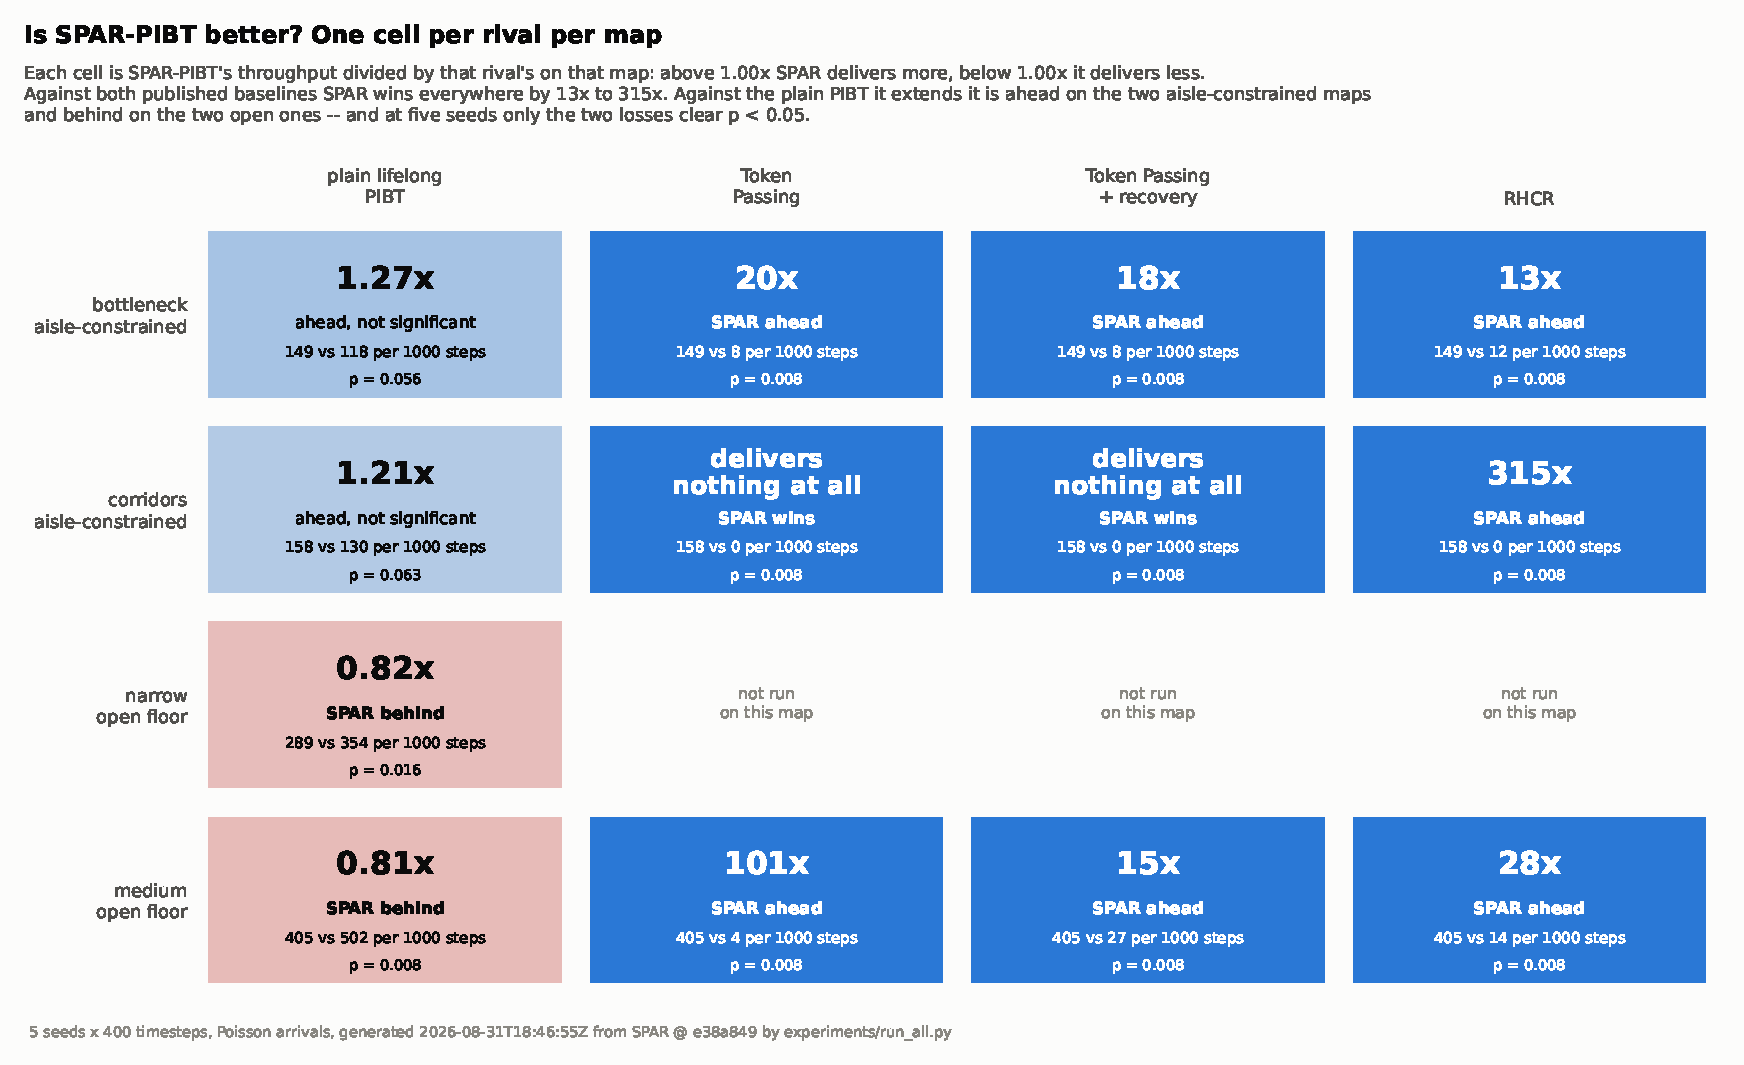
\includegraphics[width=\linewidth]{scorecard.pdf}
\caption{One cell per rival per map: SPAR-PIBT's throughput divided by that
rival's. Blue means SPAR delivers more, red means it delivers less, and the
depth of the colour is the size of the gap. This figure is the whole result;
everything after it is the explanation.}
\label{fig:scorecard}
\end{figure}

\begin{table}[H]
\centering\footnotesize
\begin{tabular}{@{}llrrrrl@{}}
\toprule
 & & \multicolumn{4}{c}{\textbf{Tasks delivered per 1000 timesteps}} & \\
\cmidrule(lr){3-6}
\textbf{Map} & \textbf{Class} & \textbf{SPAR-PIBT} & \textbf{plain PIBT} &
\textbf{TP} & \textbf{RHCR} & \textbf{Verdict for SPAR} \\
\midrule
bottleneck & aisle-constrained & \textbf{149} & 118 & 8 & 12 &
  \wins\ beats all four rivals \\
corridors & aisle-constrained & \textbf{158} & 130 & 0 & 0.5 &
  \wins\ beats all four rivals \\
narrow & open floor & 289 & \textbf{354} & --- & --- &
  \loses\ behind plain PIBT \\
medium & open floor & 405 & \textbf{502} & 27 & 14 &
  \loses\ behind plain PIBT \\
\bottomrule
\end{tabular}
\caption{The whole evaluation in one table. Throughput is stated per 1000
timesteps rather than per timestep, so 149 means 149 tasks delivered out of
every 1000 steps of simulated time. \textbf{TP} is the better of the two Token
Passing variants on that map. A dash means that baseline suite was not run on
that map. SPAR-PIBT here is the \variant{aisle\_direction\_only} configuration,
which is the best-throughput SPAR configuration on all four maps.}
\label{tab:scorecard}
\end{table}

\begin{caveat}
\textbf{How to read every number in this section.}
\begin{itemize}[leftmargin=1.2em]
\item \textbf{Throughput is tasks per 1000 timesteps} throughout this section
  and every figure. The experiment records tasks per timestep; multiplying by
  1000 changes nothing but the number of leading zeros.
\item \textbf{Higher is better} for throughput, and it is the metric that
  decides. Service time is \emph{censored} and cannot rank planners on its own
  (\Cref{fig:censoring}); cost is milliseconds per timestep, where lower is
  better.
\item \textbf{$p$ is a two-sided exact permutation test} over the same five
  seeds. Five seeds a side gives $\binom{10}{5} = 252$ label splits, so
  \textbf{the smallest attainable $p$-value is $2/252 \approx 0.008$}: a cell
  reading $p = 0.008$ is as significant as this design can report, and a
  genuine difference of moderate size can easily land at $p \approx 0.06$.
\item \textbf{Bold marks a difference at $p \leq 0.05$}; \wins\ means SPAR
  delivers more, \loses\ that it delivers less, \unclear\ that the arms are
  indistinguishable or the comparison did not run.
\item \textbf{``SPAR-PIBT'' means one fixed configuration},
  \variant{aisle\_direction\_only}, unless a table says otherwise. It is the
  best-throughput SPAR configuration on every map in this dataset, so no
  comparison in this section is cherry-picked per map.
\end{itemize}
\end{caveat}

\subsection{Setup}

Everything below comes from one dataset, \code{docs/data/}, written by
\code{experiments/run\_all.py} and committed alongside this document, so every
figure regenerates from the same runs.

\begin{table}[H]
\centering\footnotesize
\begin{tabular}{@{}lllrrl@{}}
\toprule
\textbf{Map} & \textbf{Class} & \textbf{Shape} & \textbf{Robots} &
\textbf{$\lambda$} & \textbf{Served} \\
\midrule
\variant{warehouse\_bottleneck} & aisle-constrained & two halves, one joining corridor & 16 & 0.8 & 18\% \\
\variant{warehouse\_corridors} & aisle-constrained & five parallel single-file corridors & 35 & 1.0 & 13\% \\
\variant{warehouse\_narrow} & open floor & four aisle banks, three cross-aisles & 30 & 1.2 & --- \\
\variant{warehouse\_medium} & open floor & open grid, four cross-aisles & 40 & 1.5 & 33\% \\
\bottomrule
\end{tabular}
\caption{The scenarios, and the classification used throughout this section.
\emph{Aisle-constrained} means a robot in a contended aisle has no way around
it; \emph{open floor} means cross-aisles give it one. ``Served'' is the best
planner's completed tasks over the tasks the arrival process released --- the
saturation of \Cref{sec:regime}, measured.}
\label{tab:scenarios}
\end{table}

Five seeds per cell, Poisson arrivals, and the statistics of
\Cref{sec:statistics} throughout.

\subsection{Against the published baselines}
\label{sec:results-baselines}

\begin{figure}[H]
\centering
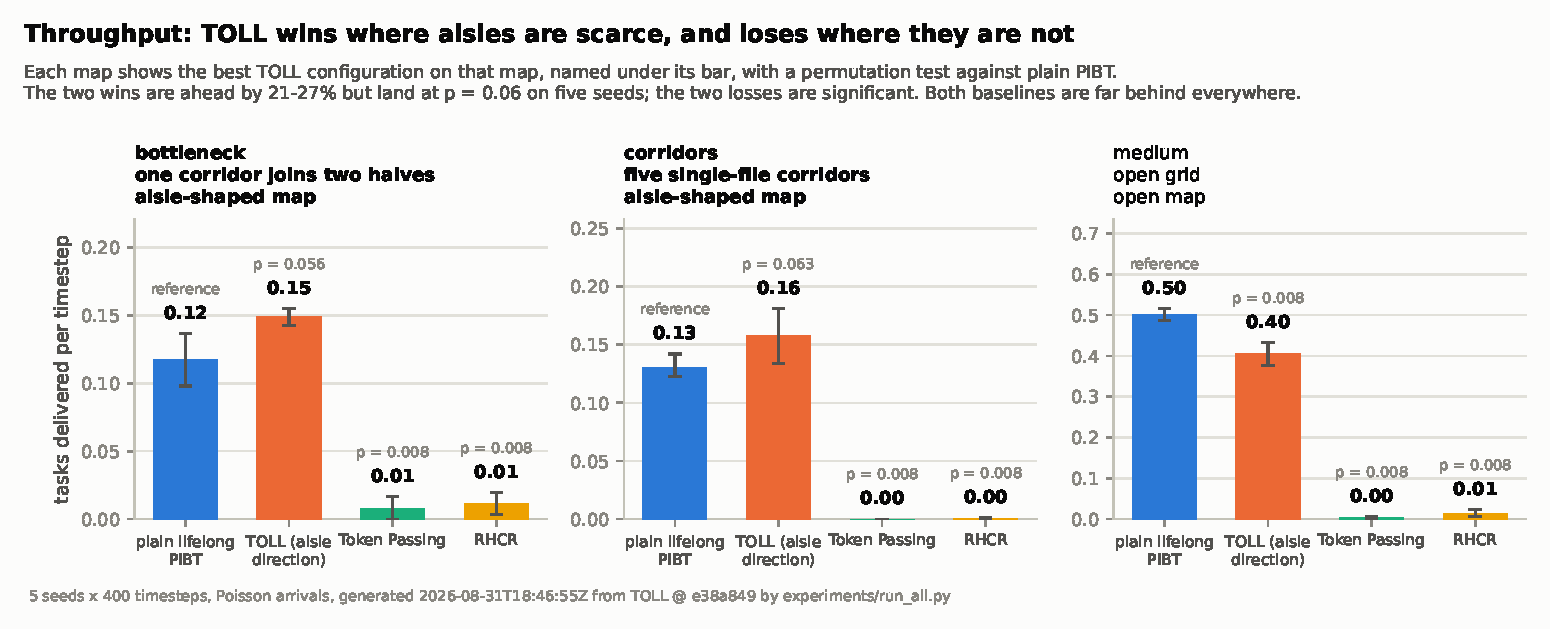
\includegraphics[width=\linewidth]{headline.pdf}
\caption{Throughput on the three maps the baseline suite covers. Both
baselines are the two short bars on every panel.}
\label{fig:headline}
\end{figure}

\begin{table}[H]
\centering\small
\begin{tabular}{@{}llrrrrl@{}}
\toprule
\textbf{Map} & \textbf{Planner} & \textbf{$\Theta_{1000}$} & \textbf{$\times$ SPAR} &
\textbf{svc} & \textbf{ms/step} & \textbf{Verdict} \\
\midrule
\multirow{5}{*}{bottleneck}
 & \textbf{SPAR-PIBT} & \textbf{149} & --- & 157 & 0.61 & --- \\
 & plain lifelong PIBT & 118 & $1.27\times$ & 154 & 0.41 & \unclear\ $p = 0.056$ \\
 & Token Passing & 8 & $19.9\times$ & 31 & 36.2 & \wins\ $p = 0.008$ \\
 & Token Passing + recovery & 8 & $17.5\times$ & 42 & 32.3 & \wins\ $p = 0.008$ \\
 & RHCR & 12 & $13.0\times$ & 23 & 75.0 & \wins\ $p = 0.008$ \\
\midrule
\multirow{5}{*}{corridors}
 & \textbf{SPAR-PIBT} & \textbf{158} & --- & 163 & 1.38 & --- \\
 & plain lifelong PIBT & 130 & $1.21\times$ & 157 & 0.82 & \unclear\ $p = 0.063$ \\
 & Token Passing & 0 & $\infty$ & --- & 80.8 & \wins\ $p = 0.008$ \\
 & Token Passing + recovery & 0 & $\infty$ & --- & 40.3 & \wins\ $p = 0.008$ \\
 & RHCR & 0.5 & $315\times$ & 9 & 43.0 & \wins\ $p = 0.008$ \\
\midrule
\multirow{5}{*}{medium}
 & \textbf{SPAR-PIBT} & 405 & --- & 158 & 1.95 & --- \\
 & plain lifelong PIBT & \textbf{502} & $0.81\times$ & 139 & 1.01 & \loses\ $p = 0.008$ \\
 & Token Passing & 4 & $101\times$ & 50 & 222.2 & \wins\ $p = 0.008$ \\
 & Token Passing + recovery & 27 & $15.0\times$ & 145 & 191.2 & \wins\ $p = 0.008$ \\
 & RHCR & 14 & $27.9\times$ & 39 & 97.9 & \wins\ $p = 0.008$ \\
\bottomrule
\end{tabular}
\caption{Five seeds, 400 timesteps. $\Theta_{1000}$ is tasks delivered per 1000
timesteps; ``$\times$ SPAR'' is SPAR-PIBT's throughput divided by that row's, so
$19.9\times$ means SPAR delivers twenty times the work; ``svc'' is mean service
time over completed tasks only (\Cref{sec:metrics}); $p$ is a two-sided
permutation test on throughput against SPAR-PIBT. A dash in the service-time
column means the planner finished no tasks at all, so the statistic does not
exist.}
\label{tab:baselines}
\end{table}

Three things in that table are worth reading carefully.

\paragraph{Both baselines lose by one to two orders of magnitude, significantly, everywhere.}
Every baseline row sits at $p = 0.008$, the floor of a five-seed test. Token
Passing completes \emph{literally zero} tasks on \variant{warehouse\_corridors}
across all five seeds. Its counters (\code{tp\_path\_not\_found},
\code{tp\_forced\_holds}) confirm genuine gridlock rather than a crash: robots
queue nose-to-tail and no robot can reserve a path through the robots ahead of
it, for the rest of the run. This is the structural failure of
\Cref{sec:related-tp}, and the first animation in \code{docs/gifs/} shows it
beside the same scenario under priority inheritance.

\paragraph{The service-time column is a trap, and this table is where it springs.}
RHCR reports a mean service time of $9$ timesteps on
\variant{warehouse\_corridors} --- easily the best figure in the table --- while
delivering half a task per 1000 timesteps. It is not fast; it is selective, and
only by accident. Token Passing's dashes are the same phenomenon taken to its
limit. \textbf{Never rank two planners by service time unless their throughputs
are comparable.}

\begin{figure}[H]
\centering
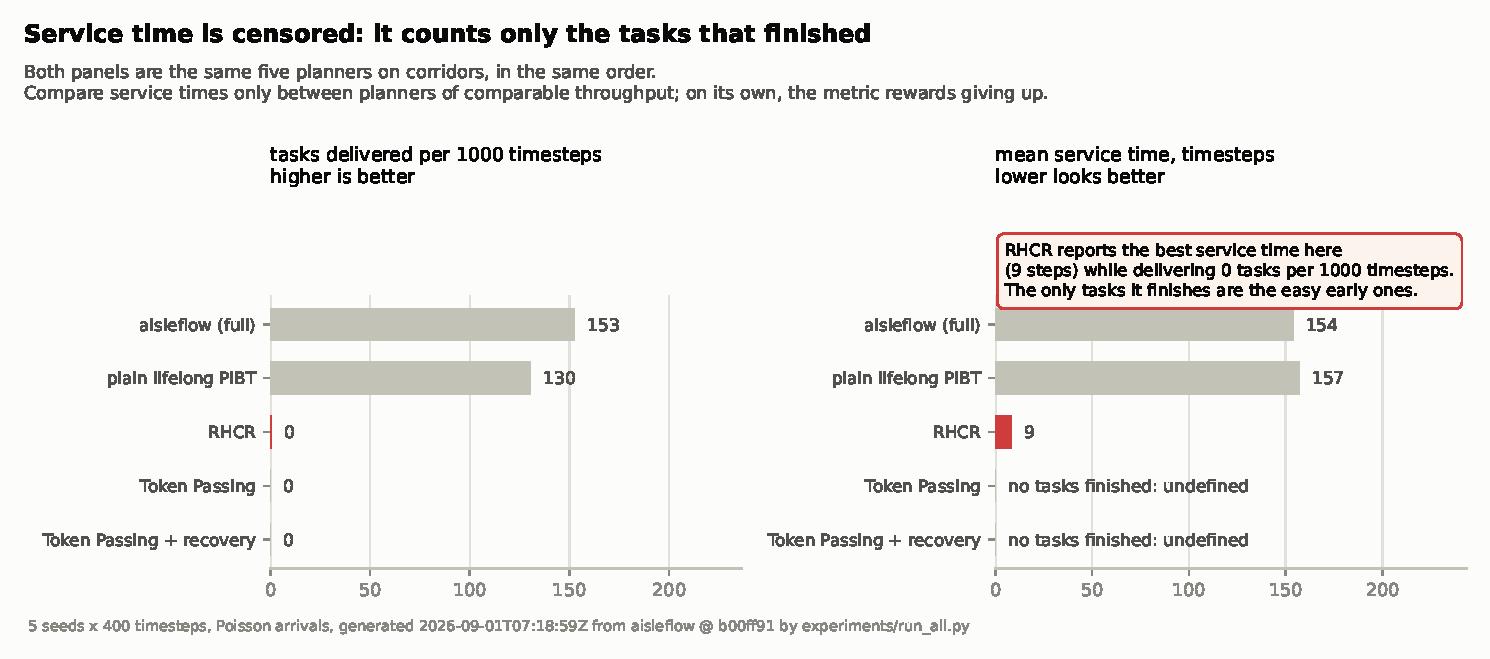
\includegraphics[width=\linewidth]{censoring.pdf}
\caption{The same five planners, twice. Ranking by the right panel alone
inverts the ranking that matters.}
\label{fig:censoring}
\end{figure}

\paragraph{Cost does not buy throughput here.}
SPAR's aisle layer costs 0.6--2.0\,ms per timestep against plain PIBT's
0.4--1.0 (4.3\,ms with every mechanism enabled); both baselines cost
32--222\,ms and deliver almost nothing at this scale.
\Cref{sec:results-caveats} states what that does and does not say about RHCR.

\begin{figure}[H]
\centering
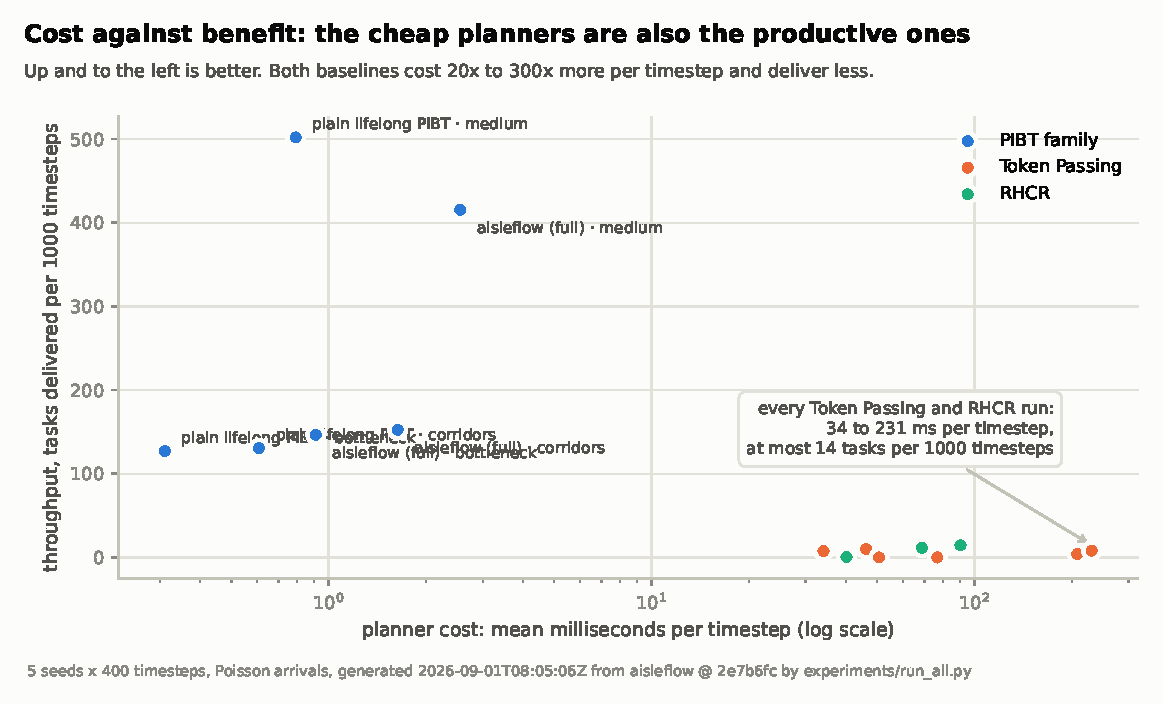
\includegraphics[width=\linewidth]{cost-benefit.pdf}
\caption{Planner cost against what it delivers; up and to the left is better.
Note the log scale on cost.}
\label{fig:cost-benefit}
\end{figure}

\subsection{Against the planner SPAR extends}
\label{sec:results-honest}

The baselines are not the hard comparison. Plain lifelong PIBT is, because
SPAR's aisle layer is built on top of it and has to earn its place there.

\begin{table}[H]
\centering\footnotesize
\begin{tabular}{@{}llrrrll@{}}
\toprule
\textbf{Map} & \textbf{Class} & \textbf{SPAR} & \textbf{plain PIBT} &
\textbf{difference} & \textbf{$p$} & \textbf{Verdict} \\
\midrule
bottleneck & aisle-constrained & \textbf{149} & 118 & $+27\%$ & 0.056 &
  \unclear\ ahead, not yet significant \\
corridors & aisle-constrained & \textbf{158} & 130 & $+21\%$ & 0.063 &
  \unclear\ ahead, not yet significant \\
narrow & open floor & 289 & \textbf{354} & $-18\%$ & 0.016 &
  \loses\ behind, significant \\
medium & open floor & 405 & \textbf{502} & $-19\%$ & 0.008 &
  \loses\ behind, significant \\
\bottomrule
\end{tabular}
\caption{The best SPAR configuration on each map --- \variant{aisle\_direction\_only}
in all four --- against plain lifelong PIBT, in tasks per 1000 timesteps. The
pattern is consistent with the design; \emph{the evidence for the winning half
of it is currently thin}, and \Cref{fig:winloss} shows the same split across
every other configuration.}
\label{tab:honest}
\end{table}

Read as evidence rather than as a headline, this table says four things.

\begin{enumerate}
\item \textbf{The split is by map class, not by map}, and it is the split the
  method predicts: the aisle layer helps where a contended aisle has no
  alternative route around it, and costs where cross-aisles already provide one.
  Four maps is four points, and \Cref{sec:results-caveats} says so.
\item \textbf{The two losses are significant; the two wins are not}
  ($p = 0.056$ and $0.063$ against $0.016$ and $0.008$). At five seeds a $+27\%$
  difference simply cannot reach the floor unless the seeds barely overlap.
  Ten seeds would settle it either way, and that is the obvious next run rather
  than a caveat to argue around.
\item \textbf{Throughput is not the only thing the aisle layer moves.} On both
  maps where it wins, it also drives about a quarter less to deliver the same
  task and halves the head-on conflicts per delivery
  (\Cref{sec:results-other-metrics}) --- effects that are significant where the
  throughput difference is not.
\item \textbf{The cost of the win is legible too}: backtracks per delivered task
  rise 85--130\% wherever an aisle commits a direction. Pricing counterflow makes
  the inheritance recursion work harder, and that is the method's largest cost.
\end{enumerate}

\begin{figure}[H]
\centering
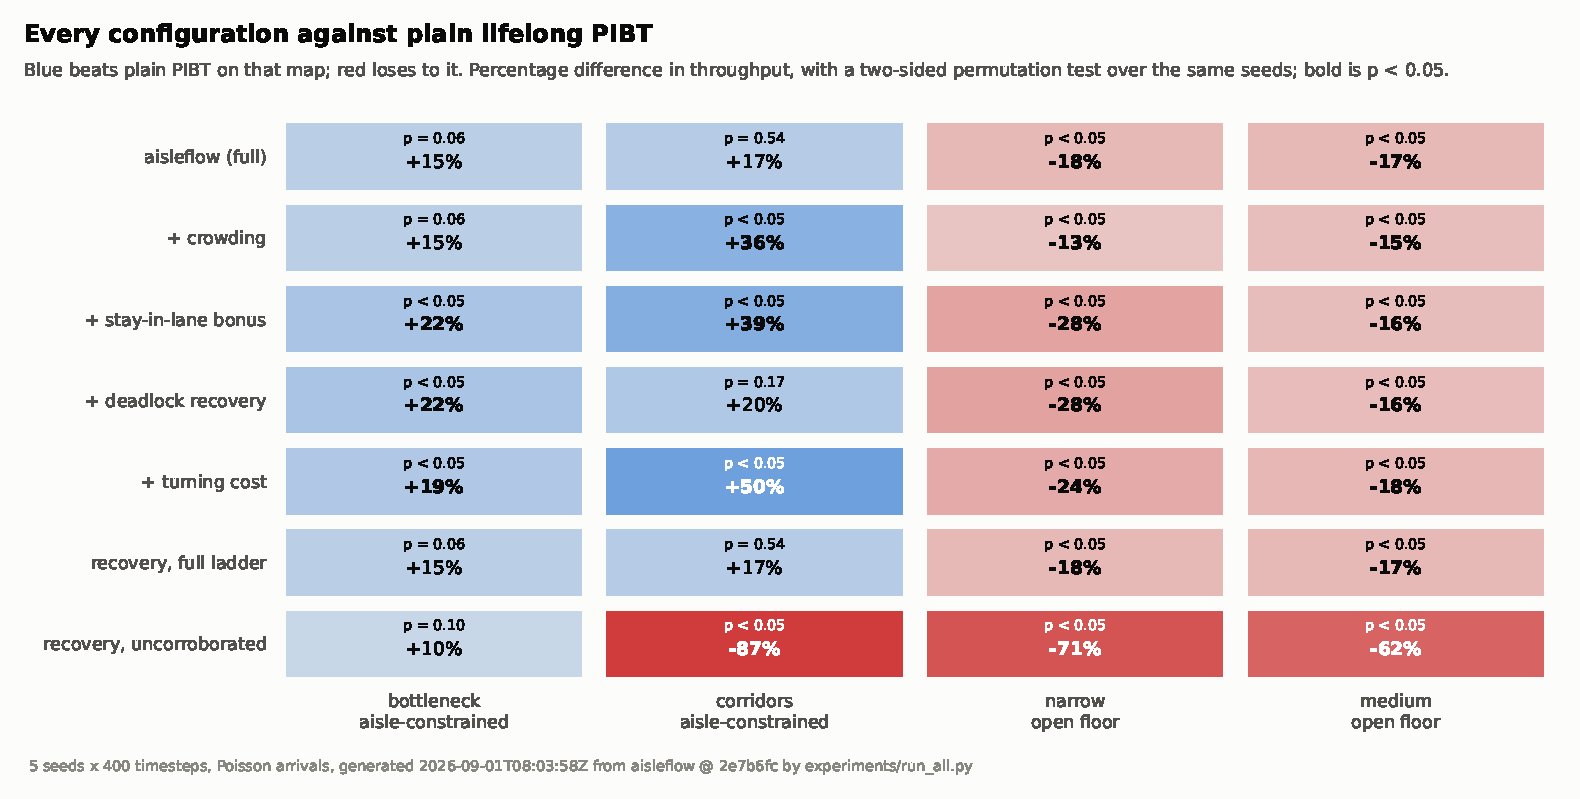
\includegraphics[width=\linewidth]{winloss.pdf}
\caption{Every configuration against plain lifelong PIBT, with a permutation
test on the same seeds. The two left columns are the aisle-constrained maps.}
\label{fig:winloss}
\end{figure}

Two rows of \Cref{fig:winloss} deserve comment. \variant{turning\_cost\_only}
--- a flat anti-zigzag penalty with nothing to do with aisles --- is the best
variant on \variant{warehouse\_corridors} (196 per 1000, $p = 0.008$) and the
second best on \variant{warehouse\_medium}. The cheapest mechanism in the system
is among the most effective, and any honest account of this work has to say so.
And on \variant{warehouse\_bottleneck} every variant beats plain PIBT by 21--28\%
while none of them clears $p = 0.05$: with no aisle ever committing a direction,
those variants differ from the base only in the turning cost, and five seeds
cannot separate them.

\subsection{Saturation, in one picture}

\begin{figure}[H]
\centering
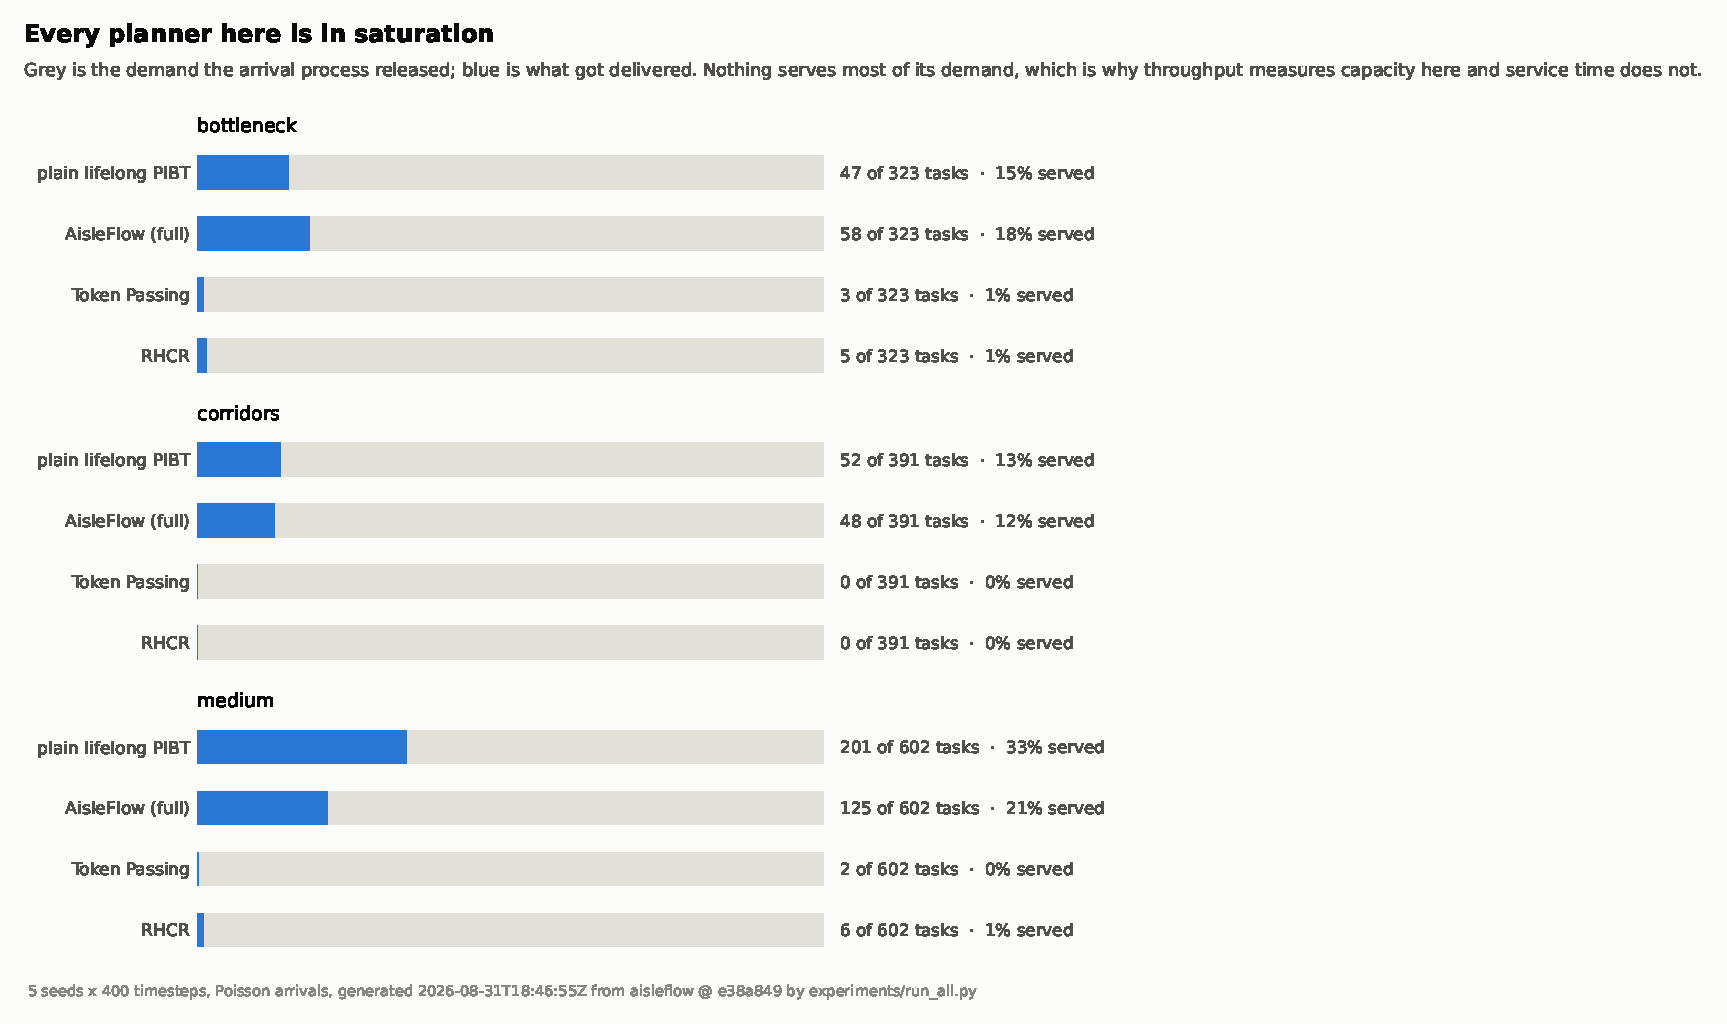
\includegraphics[width=\linewidth]{load.pdf}
\caption{Offered demand against served demand. Between 13\% and 33\% of the
tasks released are delivered; the rest are still queued when the horizon ends.}
\label{fig:load}
\end{figure}

This is \Cref{sec:regime} measured rather than asserted, and it is the context
every other number needs. Throughput here is capacity, not activity.

\subsection{Which mechanisms earn their cost}
\label{sec:results-mechanisms}

\begin{figure}[H]
\centering
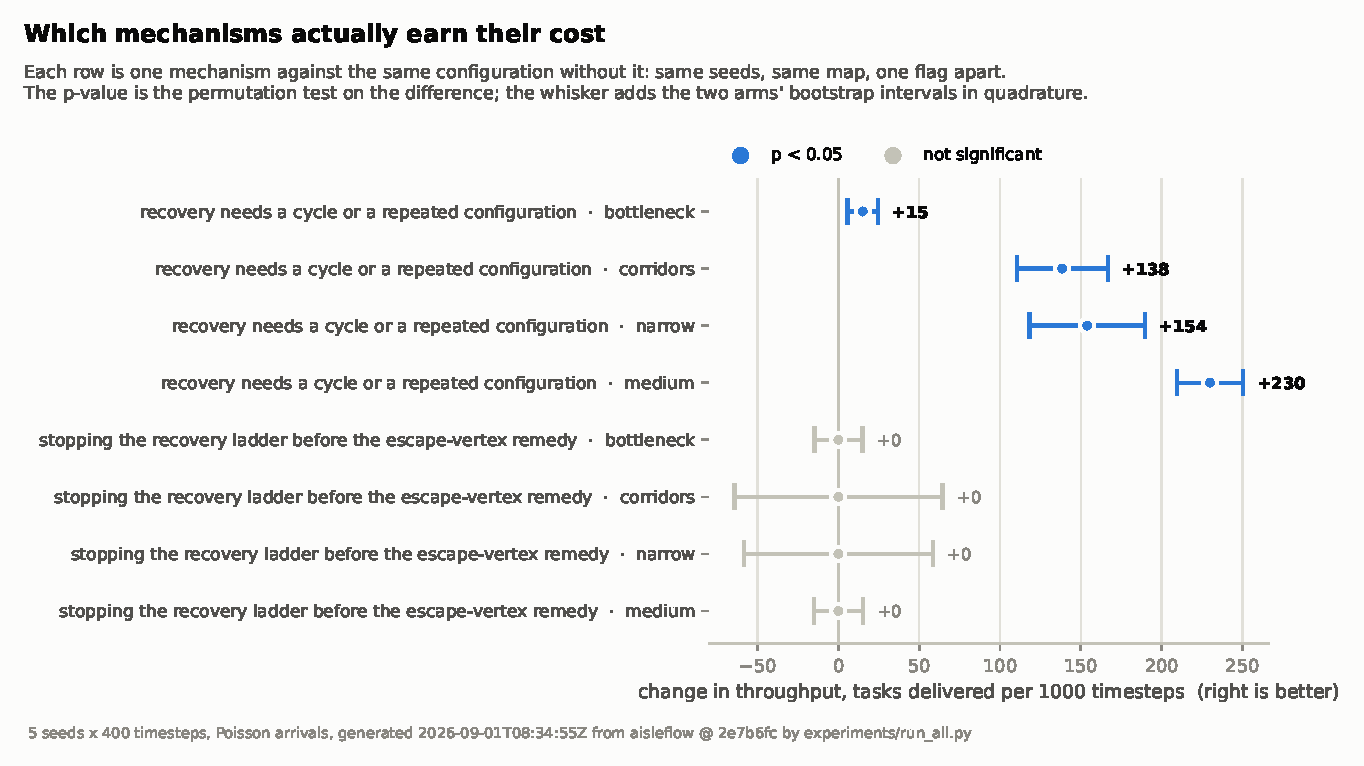
\includegraphics[width=\linewidth]{forest.pdf}
\caption{Each of the four repaired mechanisms against the same configuration
without it, on every map. Blue is $p < 0.05$.}
\label{fig:forest}
\end{figure}

\begin{table}[H]
\centering\footnotesize
\begin{tabular}{@{}lrrrr@{}}
\toprule
\textbf{Mechanism (with / without)} & \textbf{bottleneck} & \textbf{corridors} & \textbf{narrow} & \textbf{medium} \\
\midrule
direction \textbf{ranks} vs \textbf{rejects} & 149 / 149 & \textbf{158 / 84} & \textbf{289 / 78} & \textbf{405 / 161} \\
same, with reservations & \textbf{149 / 60} & \textbf{95 / 43} & \textbf{152 / 33} & 217 / 88 \\
bounded maximum green & 149 / 149 & 158 / 159 & 289 / 282 & 405 / 360 \\
recovery needs corroboration & 149 / 148 & \textbf{134 / 22} & 204 / 134 & 245 / 177 \\
\midrule
\multicolumn{5}{@{}l@{}}{\emph{as a ratio, mechanism on over mechanism off}} \\
direction \textbf{ranks} vs \textbf{rejects} & $1.0\times$ & $\mathbf{1.9\times}$ & $\mathbf{3.7\times}$ & $\mathbf{2.5\times}$ \\
same, with reservations & $\mathbf{2.5\times}$ & $\mathbf{2.2\times}$ & $\mathbf{4.6\times}$ & $2.5\times$ \\
bounded maximum green & $1.0\times$ & $1.0\times$ & $1.0\times$ & $1.1\times$ \\
recovery needs corroboration & $1.0\times$ & $\mathbf{6.1\times}$ & $1.5\times$ & $1.4\times$ \\
\bottomrule
\end{tabular}
\caption{Throughput per 1000 timesteps, with the mechanism / without it, five
seeds. \textbf{Bold} is $p \leq 0.05$. The lower block is the same rows as a
ratio, which is the form the argument uses.
\code{config.PAIRED\_DESIGNS}.}
\label{tab:mechanisms}
\end{table}

\paragraph{Direction as a price rather than a rule is the largest effect in the system.}
On the three maps where an aisle ever commits a direction it is worth
$1.9\times$ (corridors), $2.5\times$ (medium) and $3.7\times$ (narrow)
throughput, each at $p = 0.008$; with entry admission also on, the range runs
to $4.6\times$. On \variant{warehouse\_bottleneck} the two arms are identical to
three decimals, and that is not a null result: 16 robots spread over 25 aisles
never push the demand imbalance past $\tau_{\mathrm{switch}} = 5.0$, so no aisle
ever commits a direction and there is nothing for the treatment to change.
\textbf{That cell is an experiment that did not run}, and is reported as such
rather than as evidence of no effect.

This is \Cref{sec:contribution-soft} measured. The second animation in
\code{docs/gifs/} is the corridors pair, side by side.

\paragraph{Corroborated stall detection is the second.}
On \variant{warehouse\_corridors}, 134 against 22 tasks per 1000 timesteps
($p = 0.008$): a six-fold difference obtained entirely by refusing to escalate
on the weakest of the three stall signals. On the other maps the effect points
the same way and does not clear five-seed significance ($p = 0.056$ on narrow,
$0.230$ on medium). The mechanism matters most exactly where deadlocks are
easiest to manufacture.

\paragraph{The maximum green is not significant on throughput, and that is the finding.}
Its throughput effect is between $-1$ and $+45$ per 1000 timesteps, with $p$
from $0.437$ to $0.968$. It was decisive while direction was a hard constraint,
because a starved robot then had no way out at all; once counterflow is merely
expensive, a robot can buy its way out of a starved aisle and liveness no longer
rests on the signal. The two fixes are partly redundant. What the maximum green
does change is the signal itself: on \variant{warehouse\_narrow} it produces
$22.5$ direction switches per 1000 steps against $1.0$ without it
($p = 0.016$), of which $5.2$ per run are flips forced by the rule rather than
by demand (\code{starvation\_flips}). Without it, those aisles simply never turn.

\subsection{The ablation ladder is not monotone}

\begin{figure}[H]
\centering
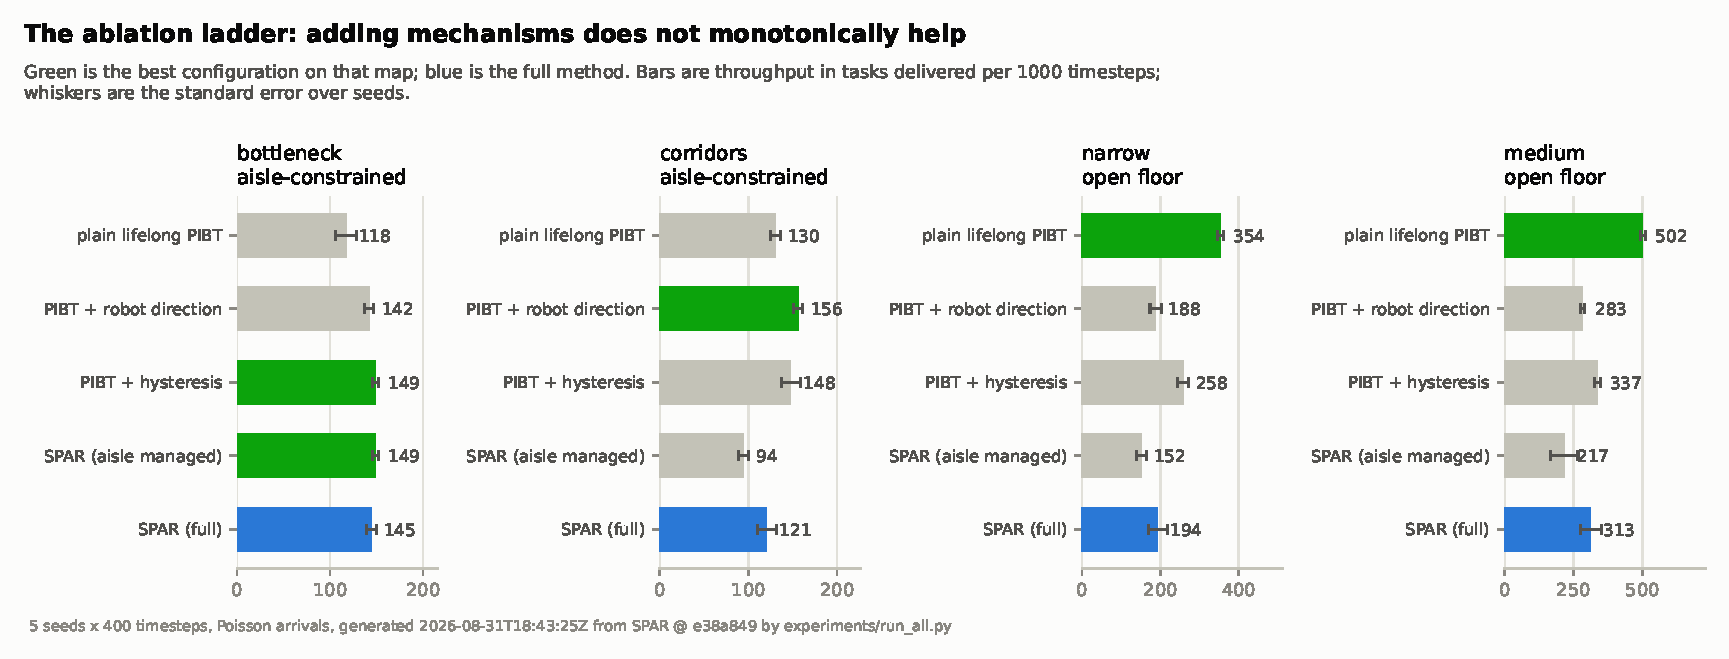
\includegraphics[width=\linewidth]{ablation-ladder.pdf}
\caption{The cumulative ladder of \Cref{sec:ablation-ladder}. Adding
mechanisms does not monotonically help, and on two maps the first rung is the
best one.}
\label{fig:ladder}
\end{figure}

This is why \Cref{tab:scorecard} reports one named configuration rather than
``the full method'': stacking every mechanism is not the best version of this
system on any map in this dataset, and saying otherwise would misrepresent it.

\subsection{Hypotheses}
\label{sec:results-hypotheses}

\begin{figure}[H]
\centering
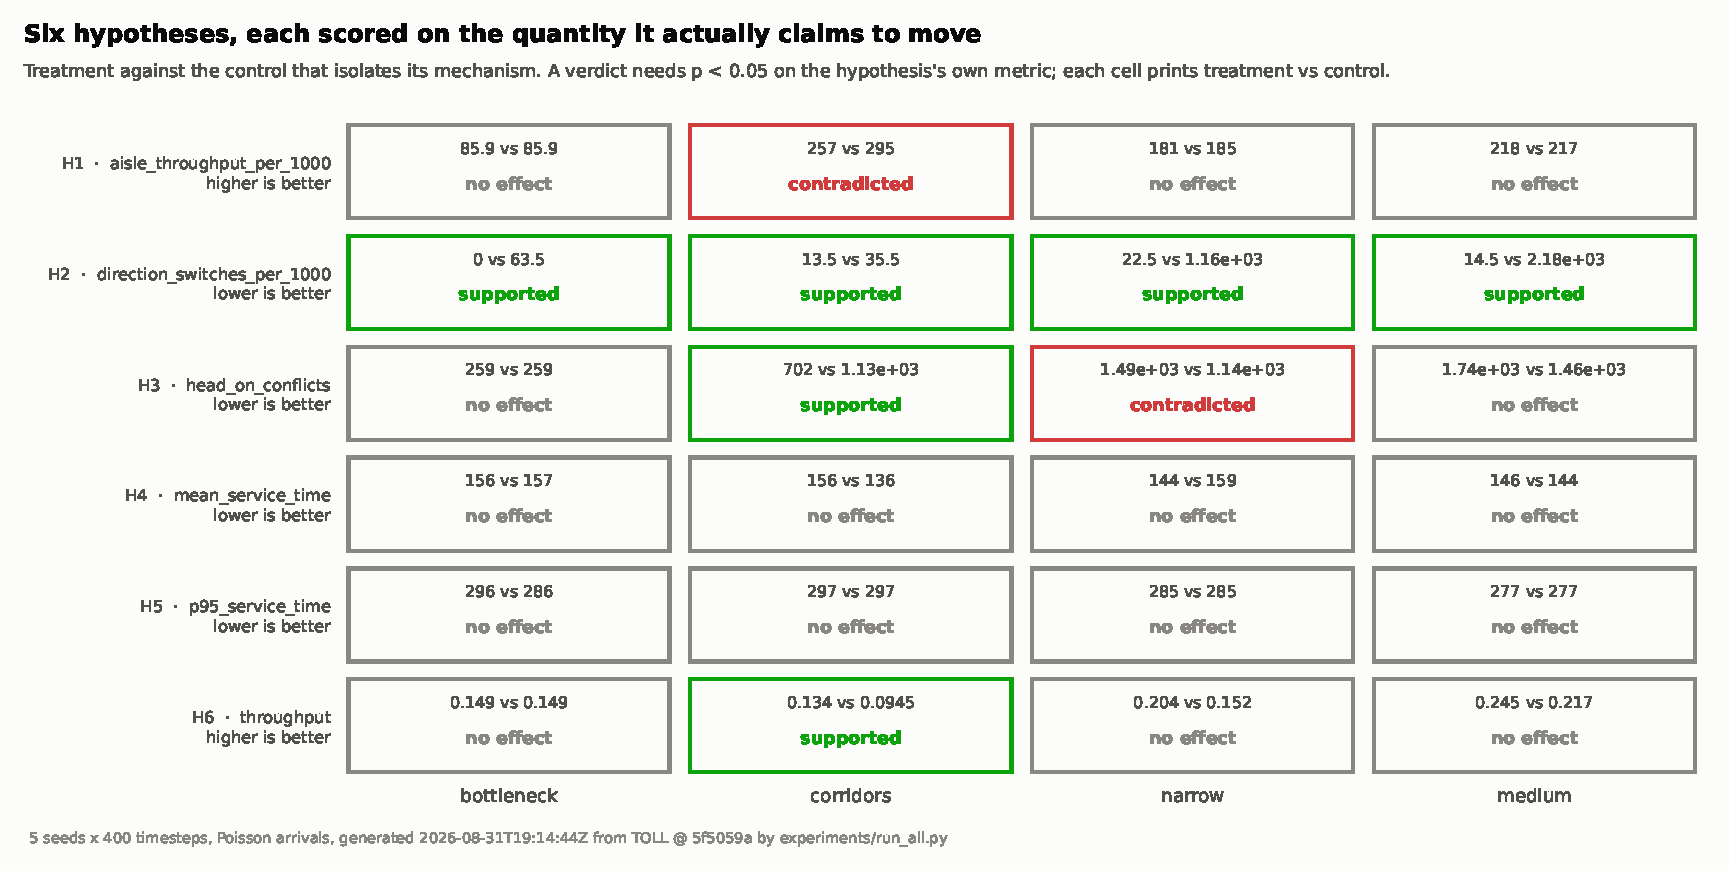
\includegraphics[width=\linewidth]{hypotheses.pdf}
\caption{Each hypothesis against the control that isolates its mechanism, on
the quantity it actually claims to move.}
\label{fig:hypotheses}
\end{figure}

Scoring each hypothesis on its own metric rather than on global throughput is
what makes these verdicts mean anything: H3 claims \emph{fewer head-on
conflicts} and H1 claims \emph{narrow aisles flow better}, and judging either by
throughput can miss a mechanism doing exactly what it promises, or credit one
that is not.

\begin{itemize}
\item \textbf{H2 (hysteresis reduces switching) is supported on every map}, at
  the five-seed floor, and by two orders of magnitude: 14.5 switches per 1000
  steps against 2188 on \variant{warehouse\_medium}.
\item \textbf{H3 (entry admission reduces head-on conflicts) is map-dependent}:
  supported on corridors (702 against 1130), contradicted on narrow. Both
  directions are real and the map decides which.
\item \textbf{H1 is contradicted on its own metric on corridors} and flat
  elsewhere, while the same configuration raises \emph{global} throughput on
  three of four maps. Both are true and not in tension: one-way aisles route
  traffic through fewer aisle transits per delivered task, so per-aisle flow
  falls while end-to-end flow rises. The lesson is about the denominator, not
  the mechanism.
\item \textbf{H5's mechanism is inert.} Changing $R_{\mathrm{near}}$ and
  $R_{\mathrm{far}}$ produces runs identical to the last decimal, because
  $\beta$ only breaks ties among candidates with \emph{equal} progress and the
  decay lowers it precisely where $\alpha \Delta$ already decides. The weight
  is not inert, and is net harmful: \variant{no\_direction\_term} ($\beta = 0$)
  beats \variant{aisle\_direction\_only} on medium (433 against 405 per 1000)
  and ties it on narrow.
\item \textbf{H4 and H6 are unsupported on three maps each}, and H6 is supported
  on corridors.
\end{itemize}

\subsection{De-confounded findings}
\label{sec:results-factorial}

The $2 \times 2$ decomposition of \Cref{eq:factorial}, on the design that could
not be read at all before the reservation layer's gating was fixed
(\Cref{sec:aisle-reservations}):

\begin{table}[H]
\centering\small
\begin{tabular}{@{}lrrrrr@{}}
\toprule
\textbf{Map} & \textbf{base} & \textbf{aisle direction} & \textbf{reservations} & \textbf{both} & \textbf{interaction} \\
\midrule
corridors & 148 & \textbf{158} & 125 & 95 & $-40$ \\
medium & 337 & \textbf{405} & 262 & 217 & $-112$ \\
\bottomrule
\end{tabular}
\caption{\code{aisle\_direction\_vs\_reservations}, tasks per 1000 timesteps.
The attribution reverses once the cells are distinct runs.}
\label{tab:factorial}
\end{table}

Aisle-level direction control is the flag that \emph{helps} in isolation
($+7\%$ and $+20\%$); entry admission is the one that costs ($-16\%$ and
$-22\%$); and the two interact strongly negatively, so the combined rung of the
ladder cannot be read as one contribution plus the other. The earlier verdict
--- direction blamed, reservations exonerated --- was reading a cell in which
factor B was a bit-identical copy of the base.

\subsection{What the other metrics say}
\label{sec:results-other-metrics}

\code{docs/metrics.md} is the companion to this section: every reported
quantity, which direction is good, and how each one misleads on its own. Three
results there are worth carrying back into this document, because they are the
clearest statement of what the aisle layer buys and what it costs, and none of
them is visible in a throughput column:

\begin{itemize}
\item \textbf{Travel distance per delivered task} falls 23\% on
  \variant{warehouse\_bottleneck} ($p = 0.008$) and 25\% on
  \variant{warehouse\_corridors} ($p = 0.016$) --- the fleet drives a quarter
  less to deliver the same task --- and rises 13\% and 21\% on the two open
  maps. The raw total is lower everywhere and means nothing: a planner that
  delivers less also drives less.
\item \textbf{Head-on conflicts per 1000 steps} fall 34\% on
  \variant{warehouse\_bottleneck} ($p = 0.016$), and 52\% per delivered task.
  That is the mechanism measured on its own terms rather than through
  throughput.
\item \textbf{Backtracks per delivered task} rise by 85--130\% wherever an
  aisle commits a direction ($p = 0.008$). Pricing counterflow makes the
  inheritance recursion explore further before it resolves, and that is the
  largest single cost of the method.
\end{itemize}

Two of these are significant on exactly the maps where the throughput
difference is not, which is the strongest form the winning claim currently
takes: \emph{on aisle-constrained maps the aisle layer demonstrably changes the
traffic in the direction it was designed to, and the throughput consequence is
consistent but not yet significant at five seeds.}

\subsection{Threats to validity}
\label{sec:results-caveats}

\begin{enumerate}
\item \textbf{Task assignment is held constant} across all five planners
  (\Cref{sec:assignment}). This isolates the movement layer, and it also means
  neither baseline was tested with the assignment policy its own paper pairs it
  with.
\item \textbf{RHCR's window and replan period (10/5) are untuned defaults}, not
  values chosen for this scale. RHCR targets hundreds of robots on much larger
  warehouses, where a rolling horizon pays for itself against full CBS. Its poor
  showing here is a property of \emph{this baseline at this scale with these
  defaults}, and is not evidence about RHCR in general.
\item \textbf{Token Passing's gridlock, by contrast, is structural} --- no
  priority inheritance, no backtracking --- and is well documented in the
  lifelong-MAPD literature. It will not go away with different hyperparameters.
\item \textbf{Five seeds is thin}, as \Cref{tab:honest} shows directly. Every
  claim of significance here rests on a test whose floor is $p = 0.008$, and
  every claim of non-significance may simply be underpowered.
\item \textbf{Four maps, one arrival process, one fleet size per map.} The
  boundary this document draws between ``aisle-constrained'' and ``open floor''
  is drawn through four points.
\end{enumerate}


\clearpage
\bibliographystyle{plainnat}
\bibliography{refs}

\end{document}
